% !TeX root = RJwrapper.tex
\title{An Open-Source Implementation of the CMPS Algorithm for Assessing Similarity of Bullets}
\author{by Wangqian Ju and Heike Hofmann}

\maketitle

\abstract{%
In this paper, we introduce the R package \pkg{cmpsR}, an open-source implementation of the Congruent Matching Profile Segments (CMPS) method developed at the National Institute of Standards and Technology (NIST) for objective comparison of striated tool marks. The functionality of the package is showcased by examples of bullet signatures that come with the package. Graphing tools are implemented in the package as well for users to assess and understand the CMPS results. Initial tests were performed on bullet signatures generated from two sets of 3D scans in the Hamby study under the framework suggested by the R package \texttt{bulletxtrctr}. New metrics based on CMPS scores are introduced and compared with existing metrics. A measure called sum of squares ratio is included, and how it can be used for evaluating different scans, metrics, or parameters is showcased with the Hamby study data sets. An open-source implementation of the CMPS algorithm makes the algorithm more accessible, generates reproducible results, and facilitates further studies of the algorithm such as method comparisons.
}

\hypertarget{introduction}{%
\subsection{Introduction}\label{introduction}}

In this paper, we present an open-source implementation of the algorithm of the Congruent Matching Profile Segments (CMPS) method.
Chen et al. (2019) developed the CMPS method for ``objective comparison of striated tool marks'' and demonstrated its use in some examples of comparing bullet signature correlations.
Although Chen et al. (2019) conceptually describe the CMPS algorithm in their paper, the authors did not release an implementation of their method.
Thus, our effort here is to introduce the CMPS method to the \texttt{R} community and provide an open-source, publicly available implementation of the algorithm to use, review, and improve.
Our implementation is made available as part of the \texttt{R} package \CRANpkg{cmpsR} on CRAN.

According to the Uniform Crime Reporting Program of the FBI (Federal Bureau of Investigation), ``more than 76 percent (76.7) of the homicides for which the FBI received weapons data in 2020 involved the use of firearms'' (United States Department of Justice, Federal Bureau of Investigation., n.d.a). At the same time, the number of murder victims jumped between 2019 and 2020 by more than 23 percent (23.4) to 17754 (United States Department of Justice, Federal Bureau of Investigation., n.d.b). This increase is unprecedented and highlights the important role that firearm examination plays in all these cases.
An important task of firearm examination is to answer the question of whether two pieces of evidence come from the same source or whether a piece of evidence matches a sample obtained from a specific firearm.
Here, in particular, we are interested to determine whether two bullets were fired from the same gun barrel.
Assessing the similarity between two bullets is based on a comparison of striation marks acquired during the firing process as bullets are propelled through the barrel.
The current state of the art sees firearms examiners make an assessment of similarity based on a visual comparison, generally, using a comparison microscope (AFTE Criteria for Identification Committee 1992).
This practice has been criticized for its lack of objectivity and the associated problem of determining valid error rates (President's Council of Advisors on Science and Technology 2016).

A report published by the Committee on Identifying the Needs of the Forensic Sciences of the National Research Council (2009) states that ``{[}m{]}uch forensic evidence-including, for example, bite marks and firearm and toolmark identification---is introduced in criminal trials without any meaningful scientific validation, determination of error rates, or reliability testing to explain the limits of the discipline.'' To overcome those criticisms and concerns, researchers have been making an effort to build databases and develop frameworks and algorithms that bring an objective and quantitative assessment into the field.
The database of Zheng (2016) with digital 3D topographic scans from various studies by Brundage (1998), Hamby, Brundage, and Thorpe (2009), Hamby et al. (2019) and others, provides a great resource for researchers. Algorithms that can be validated and tested and generate quantitative results are developed for 2D and 3D surface texture (Song et al. 2005), tool marks (Chumbley et al. 2010), and striae on Land Engraved Areas (LEAs) of bullets Chen et al. (2019).
The notion of bullet signatures is one of the results of these efforts, and we will use it to explain the CMPS algorithm and showcase the \pkg{cmpsR} implementation.
Bullet signatures can be extracted from bullet LEAs, typically one for each land engraved area, and how those bullet signatures are extracted from scans will be discussed in the Background section.
Bullet signatures capture striation marks on the bullet in a numeric format and therefore serve as the foundation for algorithms. These scans played an important role in bringing objectivity into the field.
In the following sections, we will: review the background of bullet signature comparisons, discuss how we followed the idea described by Chen et al. (2019) for the implementation of the CMPS algorithm, propose new metrics based on the CMPS score and a principled evaluation framework for algorithmic results comparison, and present results of applying our implementation to real data.

\hypertarget{background}{%
\subsection{Background}\label{background}}

\textbf{Hamby data set}

The datasets we worked with come from the James Hamby Consecutively Rifled Ruger Barrel Study (Brundage 1998; Hamby, Brundage, and Thorpe 2009; Hamby et al. 2019), in particular, Hamby set 252 and Hamby set 44.
For each Hamby set, a total of 35 bullets is fired from (the same) ten consecutively manufactured Ruger P-85 pistol barrels.
Two bullets are fired from each barrel, making up a set of 20 reference bullets.
An additional 15 bullets are fired from these ten barrels in a fashion unknown to the study participant.
The aim of the Hamby Study was to have firearms examiners identify which barrel each of the 15 questioned bullets was fired from.
The Ruger P-85 barrels are traditionally rifled barrels with six grooves and lands as shown in Figure \ref{fig:bullet}.
During the firing process, grooves and lands are engraved on a bullet.
Firearms examiners use striation marks on land engraved areas (LEAs) for their visual comparison.
For algorithmic purposes, 3D topographical images of land engraved areas were obtained and stored in x3p format (XML 3-D Surface Profile).
The x3p format provides a standard way of exchanging 2D and 3D profile data.
It conforms to \href{http://sourceforge.net/p/open-gps/mwiki/X3p/}{the ISO5436-2 standard} adopted by the OpenFMC (Open Forensic Metrology Consortium), a group of firearm forensics researchers who contributes to the establishment of best practices of using metrology in forensic science.
Hamby set 252 was scanned using a NanoFocus lens at 20x magnification with the scan resolution being 1.5625 \textmu m \(\times\) 1.5625 \textmu m per pixel.
Hamby set 44 was scanned at the Roy J Carver High-Resolution microscopy lab at Iowa State.
These scans were acquired with a Sensofar Confocal Light Microscope at 20x magnification for a nominal resolution of 0.645 \textmu m \(\times\) 0.645 \textmu m per pixel.
Both Hamby set 252 and Hamby set 44 are publicly available from the NIST Ballistics Database Project (Zheng 2016).

\textbf{Extracting signatures from LEA scans}

The automated framework for extracting signatures from x3p files used in this paper was proposed by Hare, Hofmann, and Carriquiry (2017) and is implemented in the \texttt{R} packages \CRANpkg{x3ptools} (Hofmann et al. 2020) and \texttt{bulletxtrctr} (Hofmann, Vanderplas, and Krishnan 2019).
\pkg{x3ptools} is a package to read, write, and generally, process x3p files.
The \texttt{bulletxtrctr} package implements a pipeline for extracting and comparing signatures from scans of land-engraved areas.

Figure \ref{fig:process} gives an overview of all of the steps in the process from scan to signatures.
Figure \ref{fig:process}(a) shows a rendering of a 3D scan of a bullet land engraved area.
The raised portion of the surface on the left and right of the scan are parts of the adjacent groove engraved areas (GEAs), the middle area shows a land engraved area with well expressed striation marks.
The first step of obtaining the bullet signature is to extract a cross-section at a fixed height on the land engraving.

The thin white horizontal line in Figure \ref{fig:process}(a) indicates which cross-section was identified by the algorithm to represent the LEA; Figure \ref{fig:process}(b) shows the corresponding cross-sectional view.
Groove engraved areas are removed from the analysis as indicated by the vertical blue lines in Figure \ref{fig:process}(c) and Figure \ref{fig:process}(d).
A non-parametric LOESS smooth (Cleveland, Grosse, and Shyu 1991) is fitted to capture the bullet curvature (Figure \ref{fig:process}(e)) and, finally, the \textbf{bullet signature} (Figure \ref{fig:process}(f)) is obtained as residuals of the cross-section and the fitted smooth.
Note that in Chen et al. (2019) bullet signatures are referred to as bullet profiles.
However, to avoid confusion, we distinguish the notion of bullet signatures from bullet profiles.
Bullet profiles are shown in panels (b), (c), and (d) of Figure \ref{fig:process}, while Figure \ref{fig:process}(f) shows the corresponding bullet signature.
Identifying the groove engraved areas correctly is fundamental for a correct downstream analysis of the signatures.
We have provided an interactive web application to allow for a human-in-the-middle inspection and intervention. It is implemented as an \texttt{R} Shiny App (Chang et al. 2021) named \texttt{bulletinspectR} for identifying and correcting those errors.
An example of the extraction process with corresponding code and parameter settings can be found in the ``Supplementary materials''. Note that the process of extracting signatures might be different from the one used in Chen et al. (2019) because no code or parameter settings are made available publicly.

\begin{figure}

{\centering 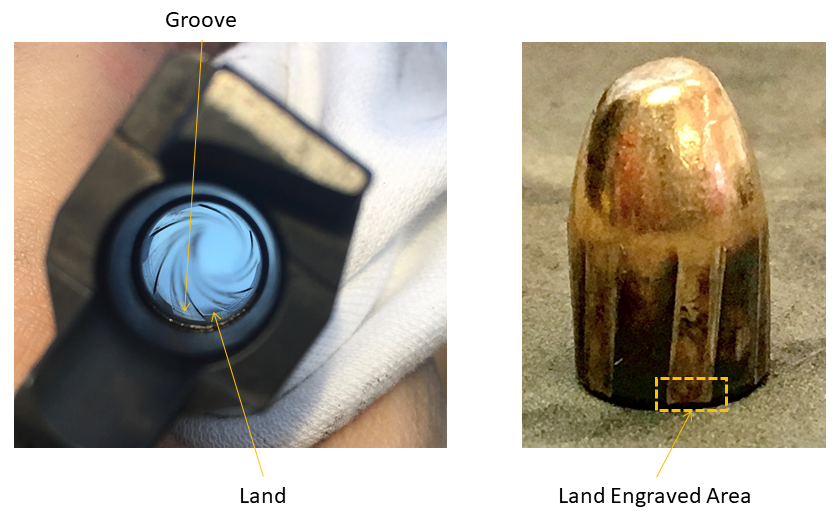
\includegraphics[width=.8\textwidth]{img/barrel_bullet_ps} 

}

\caption{Photo of a traditionally rifled gun barrel (left) and a fired bullet (right).}\label{fig:bullet}
\end{figure}

\begin{figure}

{\centering 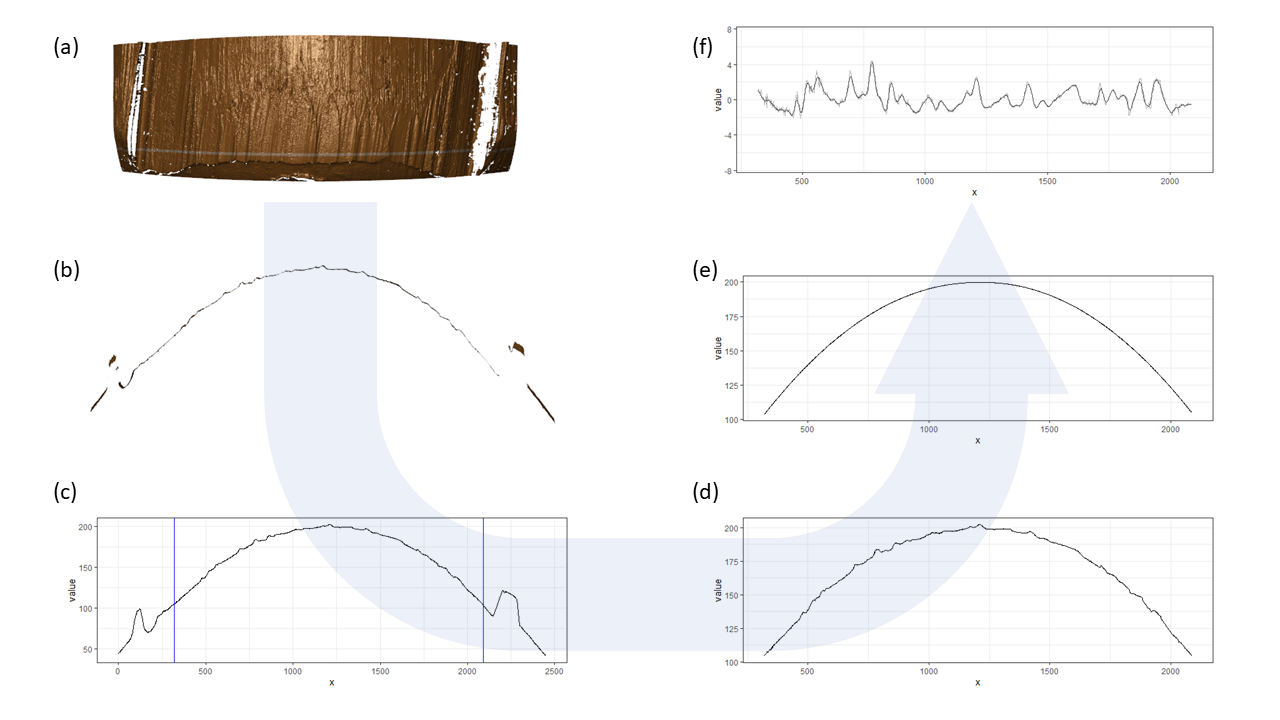
\includegraphics[width=.9\textwidth]{img/figure1_v2} 

}

\caption{A framework of obtaining a bullet signature. (a) rendering from the 3D topographic scan of a land engraved area (LEA). The selected crosscut location is indicated by a thin white horizontal line. (b) view of the cross-section of the land engraved area at the white line in (a). (c) the crosscut data plotted in 2D; blue vertical lines indicate the position of the left and right grooves. (d) the crosscut data after chopping the left and right grooves. (e) the fitted curvature using LOESS. (f) after removing the curvature from the crosscut data, the bullet signature is obtained.}\label{fig:process}
\end{figure}

\textbf{Conceptual idea of CMPS}

Most algorithms for comparing striation marks are based on the digitized signatures and produce a similarity score Krishnan and Hofmann (2019).
The congruent matching profile segments (CMPS) algorithm, developed by Chen et al. (2019) for ``objective comparison of striated tool marks'', is one such algorithm.
The algorithm's main idea is to take a set of consecutive and non-overlapping basis segments from the comparison and for each segment find the ``best'' registration position on the reference (the other bullet signature) with respect to their cross-correlation values.
From a comparison of these registration positions, a \textbf{congruent registration position} is identified, and the number of basis segments taking the congruent registration position is the CMPS score.
Note that researchers in Chen et al. (2019) refer to the origin of basis segments as the reference, but in this paper we refer to it as the comparison signature.
High CMPS scores are achieved between more similar signatures and are therefore indicative of a same-source pair.
Low scores between pairs of signatures are attributed to different source pairs.
However, a specific threshold of the CMPS score to distinguish between same-source and different-source comparisons is not provided in Chen et al. (2019), instead the threshold depends on the underlying structure of the data and the choice of parameters. In a legal setting this variability is problematic because it allows for situations in which experts could choose parameters based on whether they are witnesses for the defense or the prosecution.
Further research is needed to understand how to determine optimal threshold settings.
The CMPS algorithm can assist firearms examiners with drawing a conclusion about the source of a comparison pair.
Thus, in this paper we present an open-source implementation of the CMPS algorithm in the R package \pkg{cmpsR} available from both CRAN and Github. This publicly available implementation calculates the CMPS score of a comparison using the following code:

\begin{verbatim}
# install.packages("cmpsR")

library(cmpsR)
data(bullets)

sig1 <- bullets$sigs[[2]]$sig
sig2 <- bullets$sigs[[9]]$sig
sig3 <- bullets$sigs[[10]]$sig

cmps_result_KM <- extract_feature_cmps(sig1, sig2)
cmps_result_KNM <- extract_feature_cmps(sig1, sig3)
\end{verbatim}

In this example, the comparison between \texttt{sig1} and \texttt{sig2}, two signatures coming from the same source (a known-match comparison), gets a CMPS score of 17; the comparison between \texttt{sig1} and \texttt{sig3}, two signatures coming from different sources (a known non-match comparison), gets a CMPS score of 1.

We also implemented graphing tools for users to better understand these results as well as the algorithm itself.

The section ``Implementation'' will go through the algorithm and show how to use the \pkg{cmpsR} package.
A further example that illustrates the main points is also included.
In the section on ``Evaluation metrics'', we introduce new CMPS metrics that summarize land-level CMPS scores and a sum of squares ratio that can be used to evaluate algorithmic results.
The section ``Results'' presents the results of evaluating the \pkg{cmpsR} package using Hamby set 252 and Hamby set 44. The results from Hamby set 252 are used to verify that our implementation is, at least qualitatively, comparable to the algorithm described in Chen et al. (2019). Results from Hamby 44 show the need for a further investigation of the parameter choices even in the case of bullets fired from the same barrels.
The last section covers some final discussion and conclusions.

\hypertarget{implementation}{%
\subsection{Implementation}\label{implementation}}

\textbf{Algorithm}

Conceptually, the CMPS algorithm consists of three main steps:

\begin{enumerate}
\def\labelenumi{\arabic{enumi}.}
\item
  \textbf{cut the comparison signature into consecutive, non-overlapping, and equal-length basis segments:} The command \texttt{get\_segs(x,\ len=50)} implements this step: it takes bullet signature \texttt{x} in the format of a numeric vector and cuts it into consecutive, non-overlapping and equal-length segments of length \texttt{len}, which are referred to as ``basis segments''. Note that the parameter \texttt{len} determines the length of a basis segment and thus affects the total number of basis segments, which is the upper limit of the CMPS score of a comparison. The default value of \texttt{len} is 50, which will result in about 25 basis segments for the example data of the package.
\item
  \textbf{identify candidate positions:} For each basis segment a set of candidate registration positions on the comparison signature is identified based on the segment's similarity to the reference signature.
  In the first step, the cross-correlation function of the segment to the reference is calculated, then a number of positions with high correlation values are identified as candidate positions.
  In case multiple segment lengths are considered, the length of each basis segment is expanded (by default it is doubled) and these two steps are repeated.
  Only when candidate positions coincide (or are similar enough), they are considered further.
  Figure \ref{fig:segplots-web} and Figure \ref{fig:segplots-all-web} illustrate these ideas.

  \begin{itemize}
  \item
    \textbf{Calculate the cross-correlation curve:} Calculate the cross-correlation curve between a basis segment \texttt{x} and the reference signature \texttt{y} using the function \texttt{get\_ccf4(x,\ y,\ ...)} as shown in Figure \ref{fig:segplots-web}(b). The position indicates the lag by which a basis segment is moved with respect to its original placement. A position is considered ``good'' if it results in a peak in the cross-correlation between the basis segment and the reference.
  \item
    \textbf{Correlation peaks:} Two strategies referred to as ``multi-peak inspection'' and ``multi-peak inspection at different segment lengths'' in Chen et al. (2019) are used for identifying positions of correlation peaks as candidate positions. The latter is also called the ``multi-segment lengths strategy''. The parameter \texttt{npeaks\_set} in \texttt{extract\_feature\_cmps(...)} determines which strategy to use and the number of candidate positions:

    \begin{itemize}
    \tightlist
    \item
      If \texttt{npeaks\_set} is an integer vector of length 1, for example, \texttt{npeaks\_set\ =\ 5}, the positions of the top five peaks in the cross-correlation curve are identified as candidate positions for registration.
    \item
      If \texttt{npeaks\_set} is an integer vector of length more than 1, for example, \texttt{npeaks\_set\ =\ c(5,\ 3,\ 1)}, the multi-segment lengths strategy will be used: calculate the cross-correlation function between a basis segment and the reference and identify positions of the top five peaks; double the segment length to a specified value, re-calculate the cross-correlation function, and identify three peaks; repeat this process and identify a single peak in the newly computed cross-correlation function. Figure \ref{fig:segplots-all-web} shows an example of three levels of basis segment 6 and their corresponding cross-correlation curves and identified peaks. Note that in Chen et al. (2019) the segment length is doubled at each level of a basis segment, but in the present implementation users are allowed to choose the segment length at each level.
    \item
      \texttt{get\_ccr\_peaks(comp,\ segments,\ seg\_outlength,\ nseg\ =\ 1,\ npeaks\ =\ 5)} computes the cross-correlation curve between a basis or increased segment and the reference signature and finds peaks in the cross-correlation curve. The number of peaks detected is equal to \texttt{npeaks}, which is an integer. \texttt{segments}, \texttt{seg\_outlength}, and \texttt{nseg} determine the segment in the cross-correlation computation, and \texttt{comp} gives the reference signature. If the multi-segment lengths strategy is used, then \texttt{get\_ccr\_peaks(...)} is called in a \texttt{lapply()} for each level of the basis segment. The resulting list is called \texttt{ccr\_list}.
    \end{itemize}
  \item
    \textbf{multi-segment lengths strategy:} with the multi-segment lengths strategy being used, a position is identified as a candidate position for registration and is called a ``consistent correlation peak'' if it results in a top peak in the cross-correlation curve with a tolerance zone determined by \texttt{Tx} in all segment levels. Note that in Chen et al. (2019), a segment at its largest scale (highest level) always identifies one peak, but we do not have this requirement in our implementation.

    \begin{itemize}
    \tightlist
    \item
      the function \texttt{get\_seg\_scale(segments,\ nseg,\ out\_length)} is used to obtain the (potentially increased) version of a basis segment. \texttt{segments}, which is a list containing all basis segments generated by the function \texttt{get\_segs(...)} in step 1, and \texttt{nseg} are used to determine the basis segment to be increased. \texttt{out\_length} specifies the length of the output segment.
    \item
      \texttt{get\_ccp(ccr\_list,\ Tx\ =\ 25)} tries to identify the ``consistent correlation peak''. \texttt{ccr\_list} is the result of \texttt{lapply()} and \texttt{get\_ccr\_peaks(...)}, and \texttt{Tx} determines the size of a tolerance zone used in identifying the consistent correlation peak. \texttt{get\_ccp(...)} returns \texttt{NULL} if there is no consistent correlation peak.
    \end{itemize}
  \end{itemize}
\item
  \textbf{determine the congruent registration position:} A candidate position ``receives'' votes from basis segments that identify it or a close position within a tolerance zone of \texttt{Tx} as a candidate position in step 2.
  Votes for all candidate positions are tallied, and the position with the highest number of votes gets chosen as the \emph{congruent registration position}, indicating that most of the basis segments find their highly similar counterpart in the reference signature in terms of correlation at this registration position.
  In the case of ties, the middle position is taken as the congruent registration position.
  Basis segments with a congruent registration position are called ``congruent matching profile segments'' (CMPS).
  The total number of CMPS is the CMPS score of the comparison.
  \texttt{get\_CMPS(input\_ccp,\ Tx\ =\ 25)} is the function that tallies the votes and determines the congruent registration position and congruent matching profile segments (CMPS).
\end{enumerate}

Note that there are several parameters in the CMPS algorithm that will affect the final results and are left to the users to decide, such as the length of basis segments \texttt{seg\_length} in step 1, the number of peaks \texttt{npeaks\_set} identified on each level in step 2, and the length of the tolerance zone \texttt{Tx} in both step 2 and 3.
In our implementation of the CMPS algorithm, we used the parameters given in the original CMPS paper (Chen et al. 2019) as the default values for these parameters.
However, the authors state that no cross-validation has been done - there might also be issues with respect to the resolution of the scans.
Further research is needed, until then users are advised to think of default values as starting values and consider alternatives. However, the evaluation framework based on the sum of squares ratio introduced in the later section could be used to evaluate the choices of these parameters.
The main function that combines all steps in the CMPS algorithm described above is called \texttt{extract\_feature\_cmps(...)}.
Here we present it with its default parameters.

\begin{verbatim}
extract_feature_cmps(
  x,
  y,
  seg_length = 50,
  Tx = 25,
  npeaks_set = c(5, 3, 1),
  include = NULL,
  outlength = NULL
)
\end{verbatim}

The function \texttt{extract\_feature\_cmps} allows for the following input from users besides the previously discussed parameters \texttt{seg\_length}, \texttt{npeaks\_set}, and \texttt{Tx}:

\begin{itemize}
\item
  \texttt{x} and \texttt{y} are two signatures: \texttt{x} serves as the comparison signature (which will be divided into basis segments) and \texttt{y} is the reference signature;
\item
  \texttt{include} determines the format of the function result.
  Besides the \texttt{CMPS\_score}, other aspects of the comparison help in understanding how the \texttt{CMPS\_score} is computed.
  By default \texttt{include} is set to \texttt{NULL} and only the \texttt{CMPS\_score} is returned; further results are included when \texttt{include} is (an abbreviation of) one of or a vector of the following strings: \texttt{"nseg"}, \texttt{"congruent\_pos"}, \texttt{"congruent\_seg\_idx"}, \texttt{"segments"}, \texttt{"parameters"}, and \texttt{"full\_result"}.
  If \texttt{include} is specified as \texttt{"full\_result"} (or its abbreviation), the output includes everything listed below.

  \begin{itemize}
  \tightlist
  \item
    \texttt{nseg}: the number of basis segments from the comparison signature; this is also the highest possible CMPS score of the comparison;
  \item
    \texttt{congruent\_pos}: the congruent registration position;
  \item
    \texttt{congruent\_seg\_idx}: the indices of all congruent matching profile segments;
  \item
    \texttt{ccp\_list}: a list showing identified candidate positions of all basis segments;
  \item
    \texttt{pos\_df}: a data frame containing all candidate positions and their respective number of votes;
  \item
    \texttt{segments}: a list containing all basis segments;
  \item
    \texttt{parameters}: a list containing all input arguments of \texttt{extract\_feature\_cmps};
  \end{itemize}
\item
  \texttt{outlength} specifies the segment length of a basis segment at each level under the multi-segment lengths strategy.
  By default \texttt{outlength} is set to \texttt{NULL}, indicating that a basis segment should double its segment length at the next level and conforming to the description in Chen et al. (2019) .
\end{itemize}

In the remainder of the paper, we showcase the use of the \pkg{cmpsR} functionality on some examples and present the results of applying it to two datasets.

\textbf{Installation}

The \pkg{cmpsR} package is publicly available from CRAN and can be installed by

\begin{verbatim}
install.packages("cmpsR")
\end{verbatim}

Moreover, its development version is also available from Github and can be installed by

\begin{verbatim}
# install.packages("remotes")
remotes::install_github("willju-wangqian/cmpsR")
\end{verbatim}

\textbf{An example}

The \pkg{cmpsR} package contains a simple example to illustrate the basic usage of the package.
The data in this example are twelve bullet signatures obtained from two bullets in Hamby set 252 (Hamby, Brundage, and Thorpe 2009).
The procedure for generating signatures from high-resolution 3D topographic scans of bullet lands used here follows the methodology described in Hare, Hofmann, and Carriquiry (2017) (as discussed above).
The two bullets under consideration are known to have been fired from the same gun barrel, so for the 36 pairwise land-by-land comparisons, six comparisons are from same-source pairs (known matches) while thirty are from different-source pairs (known non-matches).
To access the example data, we use

\begin{verbatim}
library(cmpsR)
data(bullets)
\end{verbatim}

\texttt{bullets\$sigs} is a list of twelve numeric vectors corresponding to the twelve bullet signatures shown in Figure \ref{fig:sigs}.
\texttt{bullets\$source} contains the URLs to the corresponding x3p file containing the topographic scan from the NIST Ballistics Toolmark Research Database (Zheng 2016).

\begin{figure}

{\centering 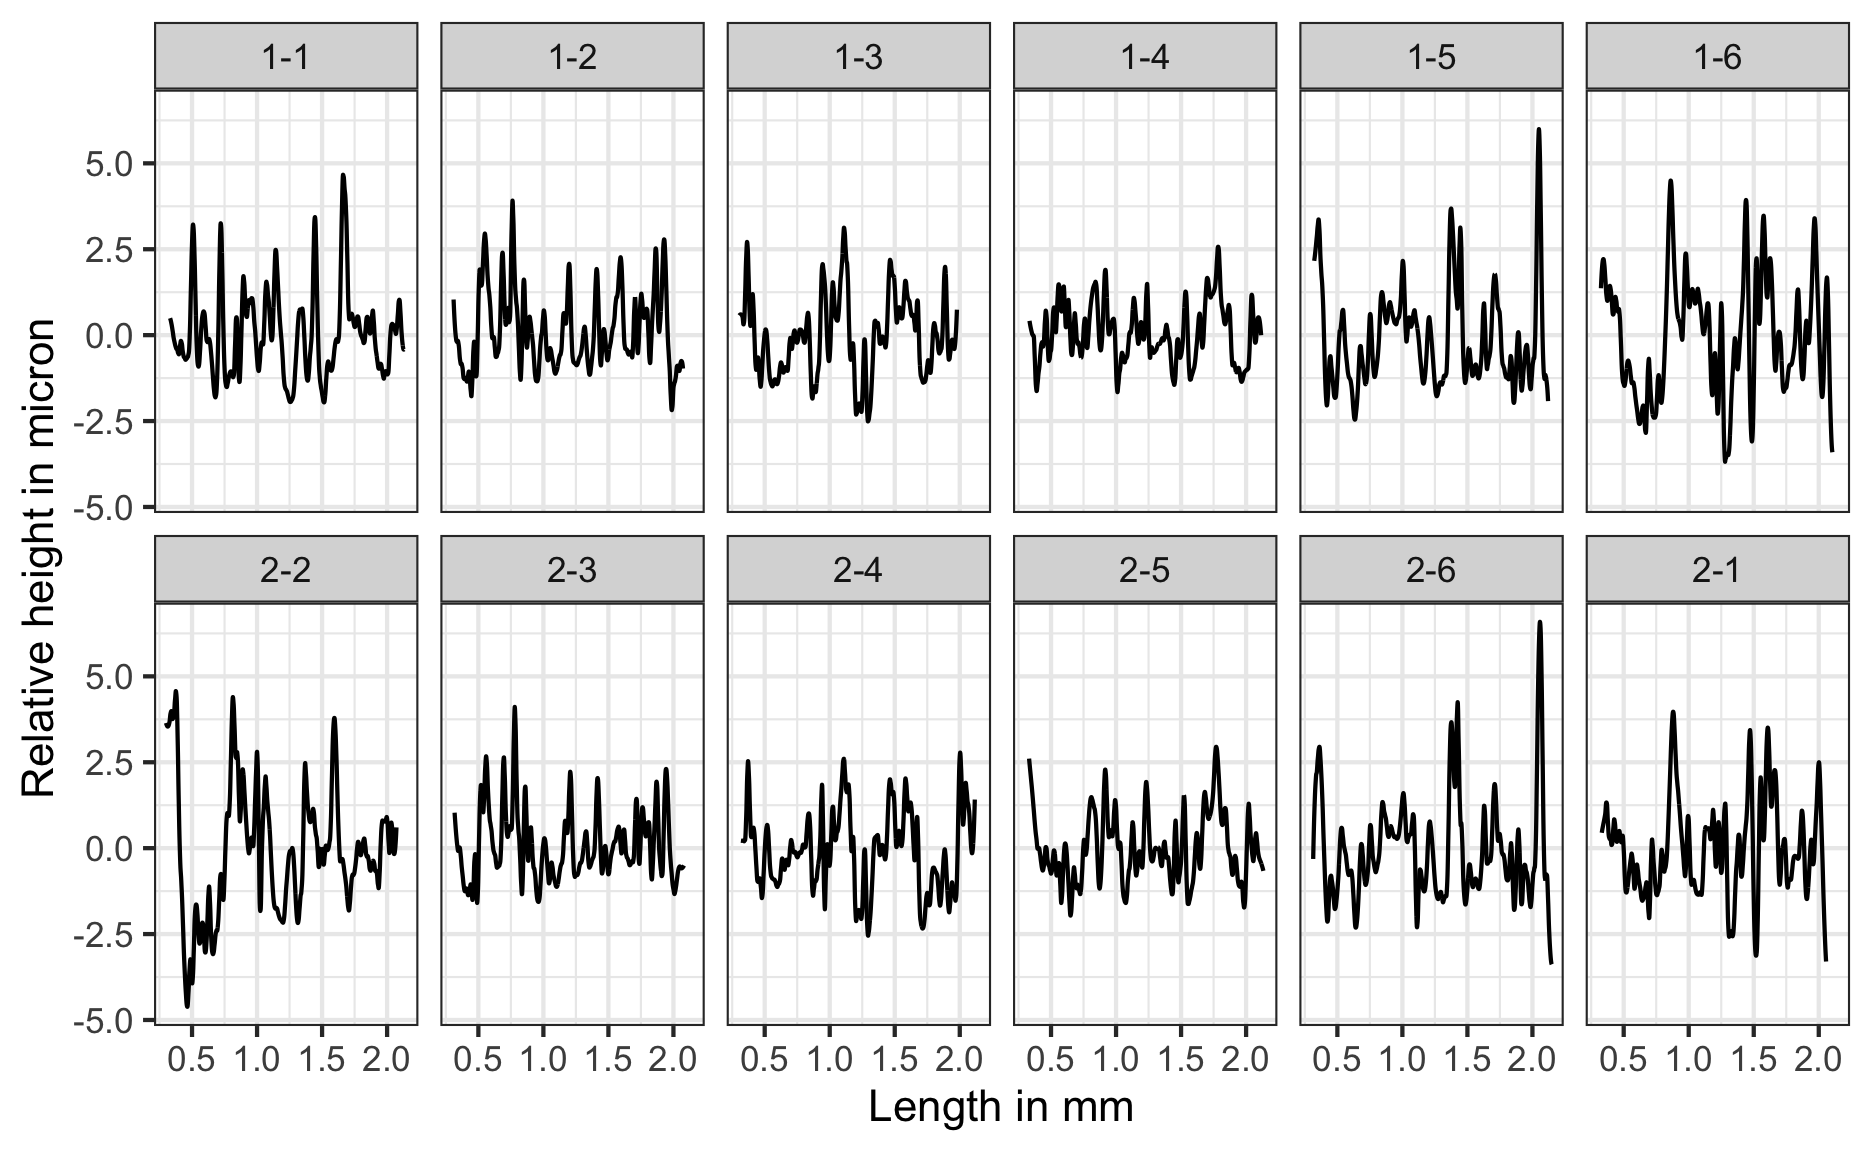
\includegraphics[width=\textwidth]{RJ-2022-035_files/figure-latex/sigs-1} 

}

\caption{Signatures of all lands of bullet 1 in the top row, and of bullet 2 in the bottom row. Signatures in the second row are ordered to be in phase with the signatures above, i.e. matching signatures are displayed on top of each other. On the x-axis is the length of the scan in millimeter, and on the y-axis is the relative height in micron.}\label{fig:sigs}
\end{figure}

The signatures of Land 4 of Bullet 1 and Land 5 of Bullet 2 are stored in objects \texttt{sigs2} and \texttt{sigs1}, respectively.
This comparison consists of a pair of signatures that are known to be a match -- a KM (known match) comparison.
We compute the CMPS score using two versions of the CMPS algorithm:

\begin{verbatim}
sigs1 <- bullets$sigs[bullets$bulletland == "2-5"][[1]]
sigs2 <- bullets$sigs[bullets$bulletland == "1-4"][[1]]

# compute cmps

# algorithm with multi-peak insepction at three different segment levels
cmps_with_multi_scale <-
  extract_feature_cmps(sigs1$sig, sigs2$sig,
    npeaks_set = c(5, 3, 1), include = "full_result"
  )

# algorithm with multi-peak inspection at the basis scale only
cmps_without_multi_scale <-
  extract_feature_cmps(sigs1$sig, sigs2$sig,
    npeaks_set = 5, include = "full_result"
  )
\end{verbatim}

In the first example, \texttt{npeaks\_set} is a vector of three integers, i.e.~the algorithm uses the multi-segment lengths strategy to create the result object \texttt{cmps\_with\_multi\_scale}.
For \texttt{cmps\_without\_multi\_scale} each basis segment is linked to the top 5 candidate positions.
We use \texttt{include\ =\ "full\_result"} to capture all results.
In this example, the CMPS is 9 when using multiple segments, and 12 when using a single segment.
As discussed in Chen et al. (2019), using multi-segment lengths strategy can reduce the number of false positives when identifying candidate positions; however, any score-based method is walking the line between false positives and false negatives.
As the number of false positives is reduced the number of false negatives might rise.
More discussion and comparisons between the two versions of the CMPS algorithm will be presented in later sections.
Note that the multi-segment lengths method is slower because the algorithm is run once for each segment length.

\textbf{Visualize and understand CMPS results}

We also implemented graphing tools for visualizing the results of the CMPS algorithm.
The goal is to provide users with tools to inspect each of the basis segments and to help them have a better understanding of how the algorithm works.
Figure \ref{fig:sigplots-web} shows the plots generated by the first graphing function, \texttt{cmps\_signature\_plot()}, and continues with the example above.
\texttt{cmps\_signature\_plot()} takes the output of \texttt{extract\_feature\_cmps(...,\ include\ =\ "full\_result")} and returns a list of 5 elements.
It creates an overall impression of how the comparison signature aligns with the reference signature at the congruent registration position.

\begin{itemize}
\item
  The first element is a plot called \texttt{segment\_shift\_plot}, shown in Figure \ref{fig:sigplots-web}(a). On this plot the reference signature is drawn as a black line, congruent matching profile segments from the comparison signature are overlaid in red at the congruent registration position.

\begin{verbatim}
sig_plot <- cmps_signature_plot(
  cmps_with_multi_scale
)

# (a)
sig_plot$segment_shift_plot
\end{verbatim}
\item
  The second plot is called \texttt{signature\_shift\_plot}, shown in Figure \ref{fig:sigplots-web}(b). This visual presents both the comparison signature and the reference signature. The comparison signature is aligned with the reference signature based on the congruent registration position. Congruent matching profile segments are highlighted by solid red lines.

\begin{verbatim}
# (b)
sig_plot$signature_shift_plot
\end{verbatim}
\end{itemize}

\begin{figure}

{\centering 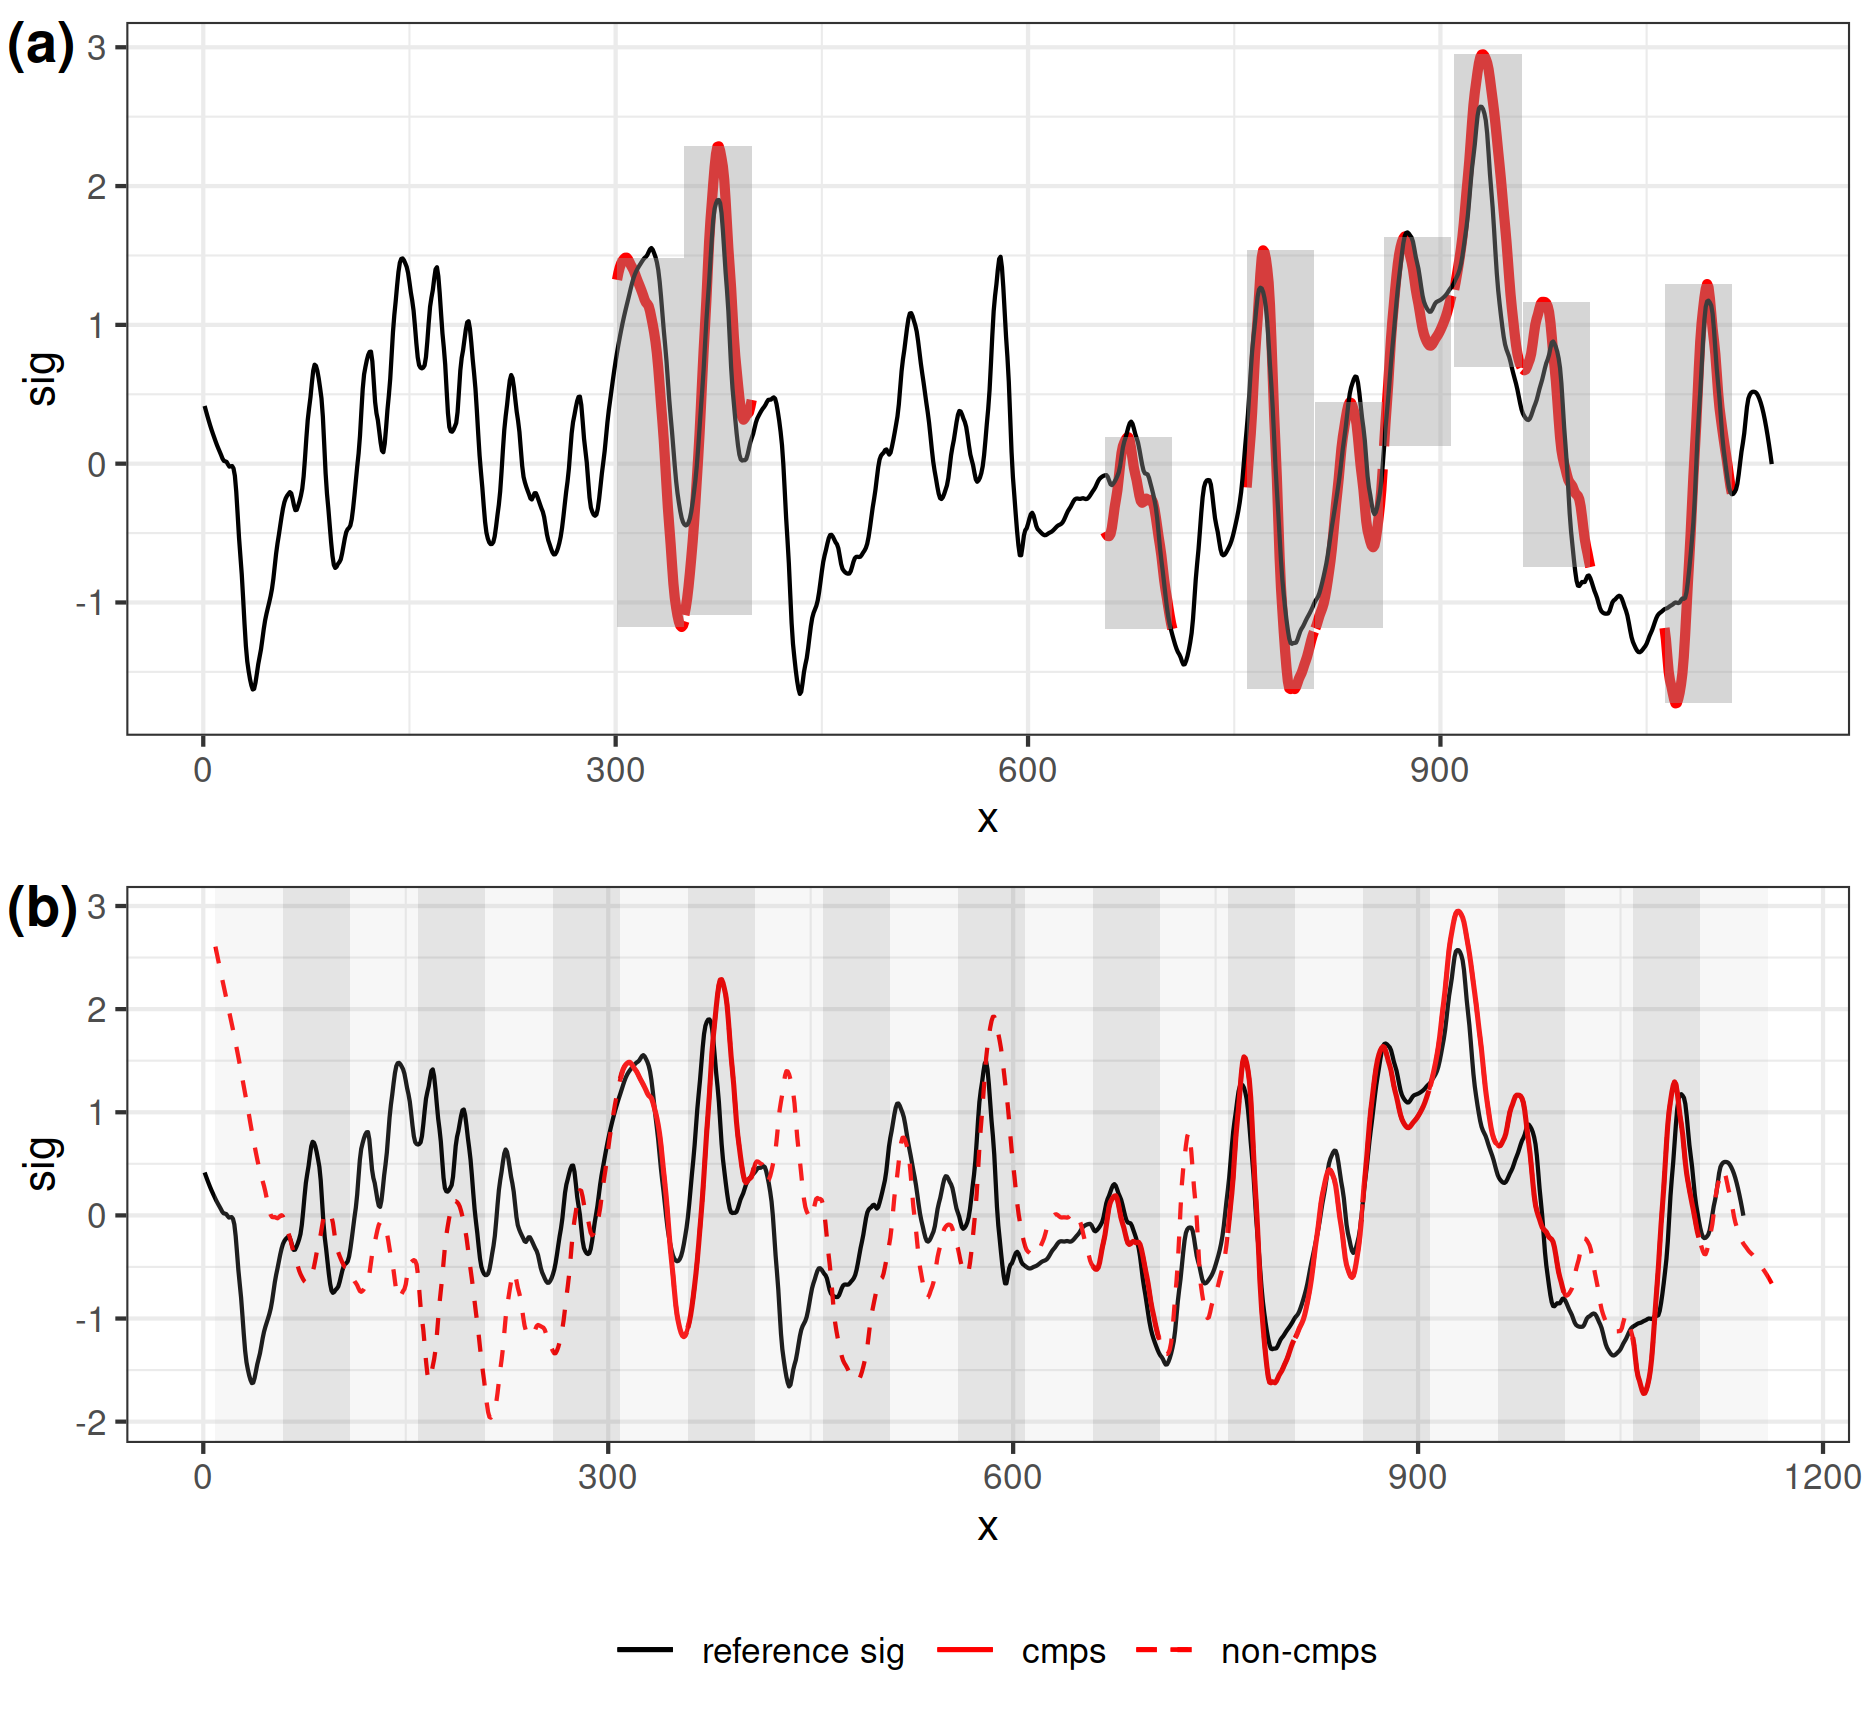
\includegraphics[width=.7\textwidth]{RJ-2022-035_files/figure-latex/sigplots-web-1} 

}

\caption{In (a) the black line shows the comparison signature; each red line segment shows one congruent matching profile segment. Each grey rectangle highlights one congruent matching profile segment. In (b) the black line shows the reference signature; the red line shows the comparison signature. Solid part shows the congruent matching profile segments, and the dashed part shows segments that do not agree with the congruent registration position.}\label{fig:sigplots-web}
\end{figure}

\begin{itemize}
\tightlist
\item
  Other elements of this list are \texttt{seg\_shift} and \texttt{sig\_shift}. \texttt{sig\_shift} gives the congruent registration position, while \texttt{seg\_shift} is a data frame showing the congruent matching profile segments and their identified candidate position closest to the congruent registration position.
\end{itemize}

\begin{verbatim}
sig_plot$seg_shift
#>    seg_idx seg_shift
#> 7        7         0
#> 8        8        -1
#> 14      14         5
#> 16      16         8
#> 17      17         8
#> 18      18         8
#> 19      19         9
#> 20      20         9
#> 22      22        12
\end{verbatim}

While \texttt{cmps\_signature\_plot()} focuses on the signature level, \texttt{cmps\_segment\_plot()} focuses on the segment level.
It provides the ``full result'' of \texttt{extract\_feature\_cmps()}, but also takes an argument, \texttt{seg\_idx}, indicating which segment should be inspected.
When checking \texttt{sig\_plot\$seg\_shift} we notice that segment number 6 is not one of the congruent matching profile segments.
We can therefore set \texttt{seg\_idx\ =\ 6} in \texttt{cmps\_segment\_plot()} and investigate the reason why this segment disagrees with the congruent registration position.

For each segment scale, we have two plots: \texttt{segment\_plot} and \texttt{scale\_ccf\_plot}, as shown in Figure \ref{fig:segplots-web} for the example of segment number 6:

\begin{itemize}
\item
  Figure \ref{fig:segplots-web}(a) is the \texttt{segment\_plot} for basis segment 6 at level one (in its original length). We used \texttt{npeaks\_set\ =\ c(5,\ 3,\ 1)} in \texttt{extract\_feature\_cmps()} when calculating the CMPS score. Therefore the top five peaks are identified in the cross-correlation curve at level one. Segment 6 is plotted at the positions where these five peaks are identified with dashed lines in the \texttt{segment\_plot}. The solid thick black line shows the segment at its original position (which in this example is very close to the actual registration position).

\begin{verbatim}
seg_plot <- cmps_segment_plot(
  cmps_with_multi_scale,
  seg_idx = 6
)

# (a)
seg_plot[[1]]$segment_plot
\end{verbatim}
\item
  Figure \ref{fig:segplots-web}(b) is the \texttt{scale\_ccf\_plot} of basis segment 6 at level one. It shows the cross-correlation curve computed by the reference signature and the level-one basis segment 6. The five highest peaks are marked by dots on the curve.

\begin{verbatim}
# (b)
seg_plot[[1]]$scale_ccf_plot
\end{verbatim}
\end{itemize}

\begin{figure}

{\centering 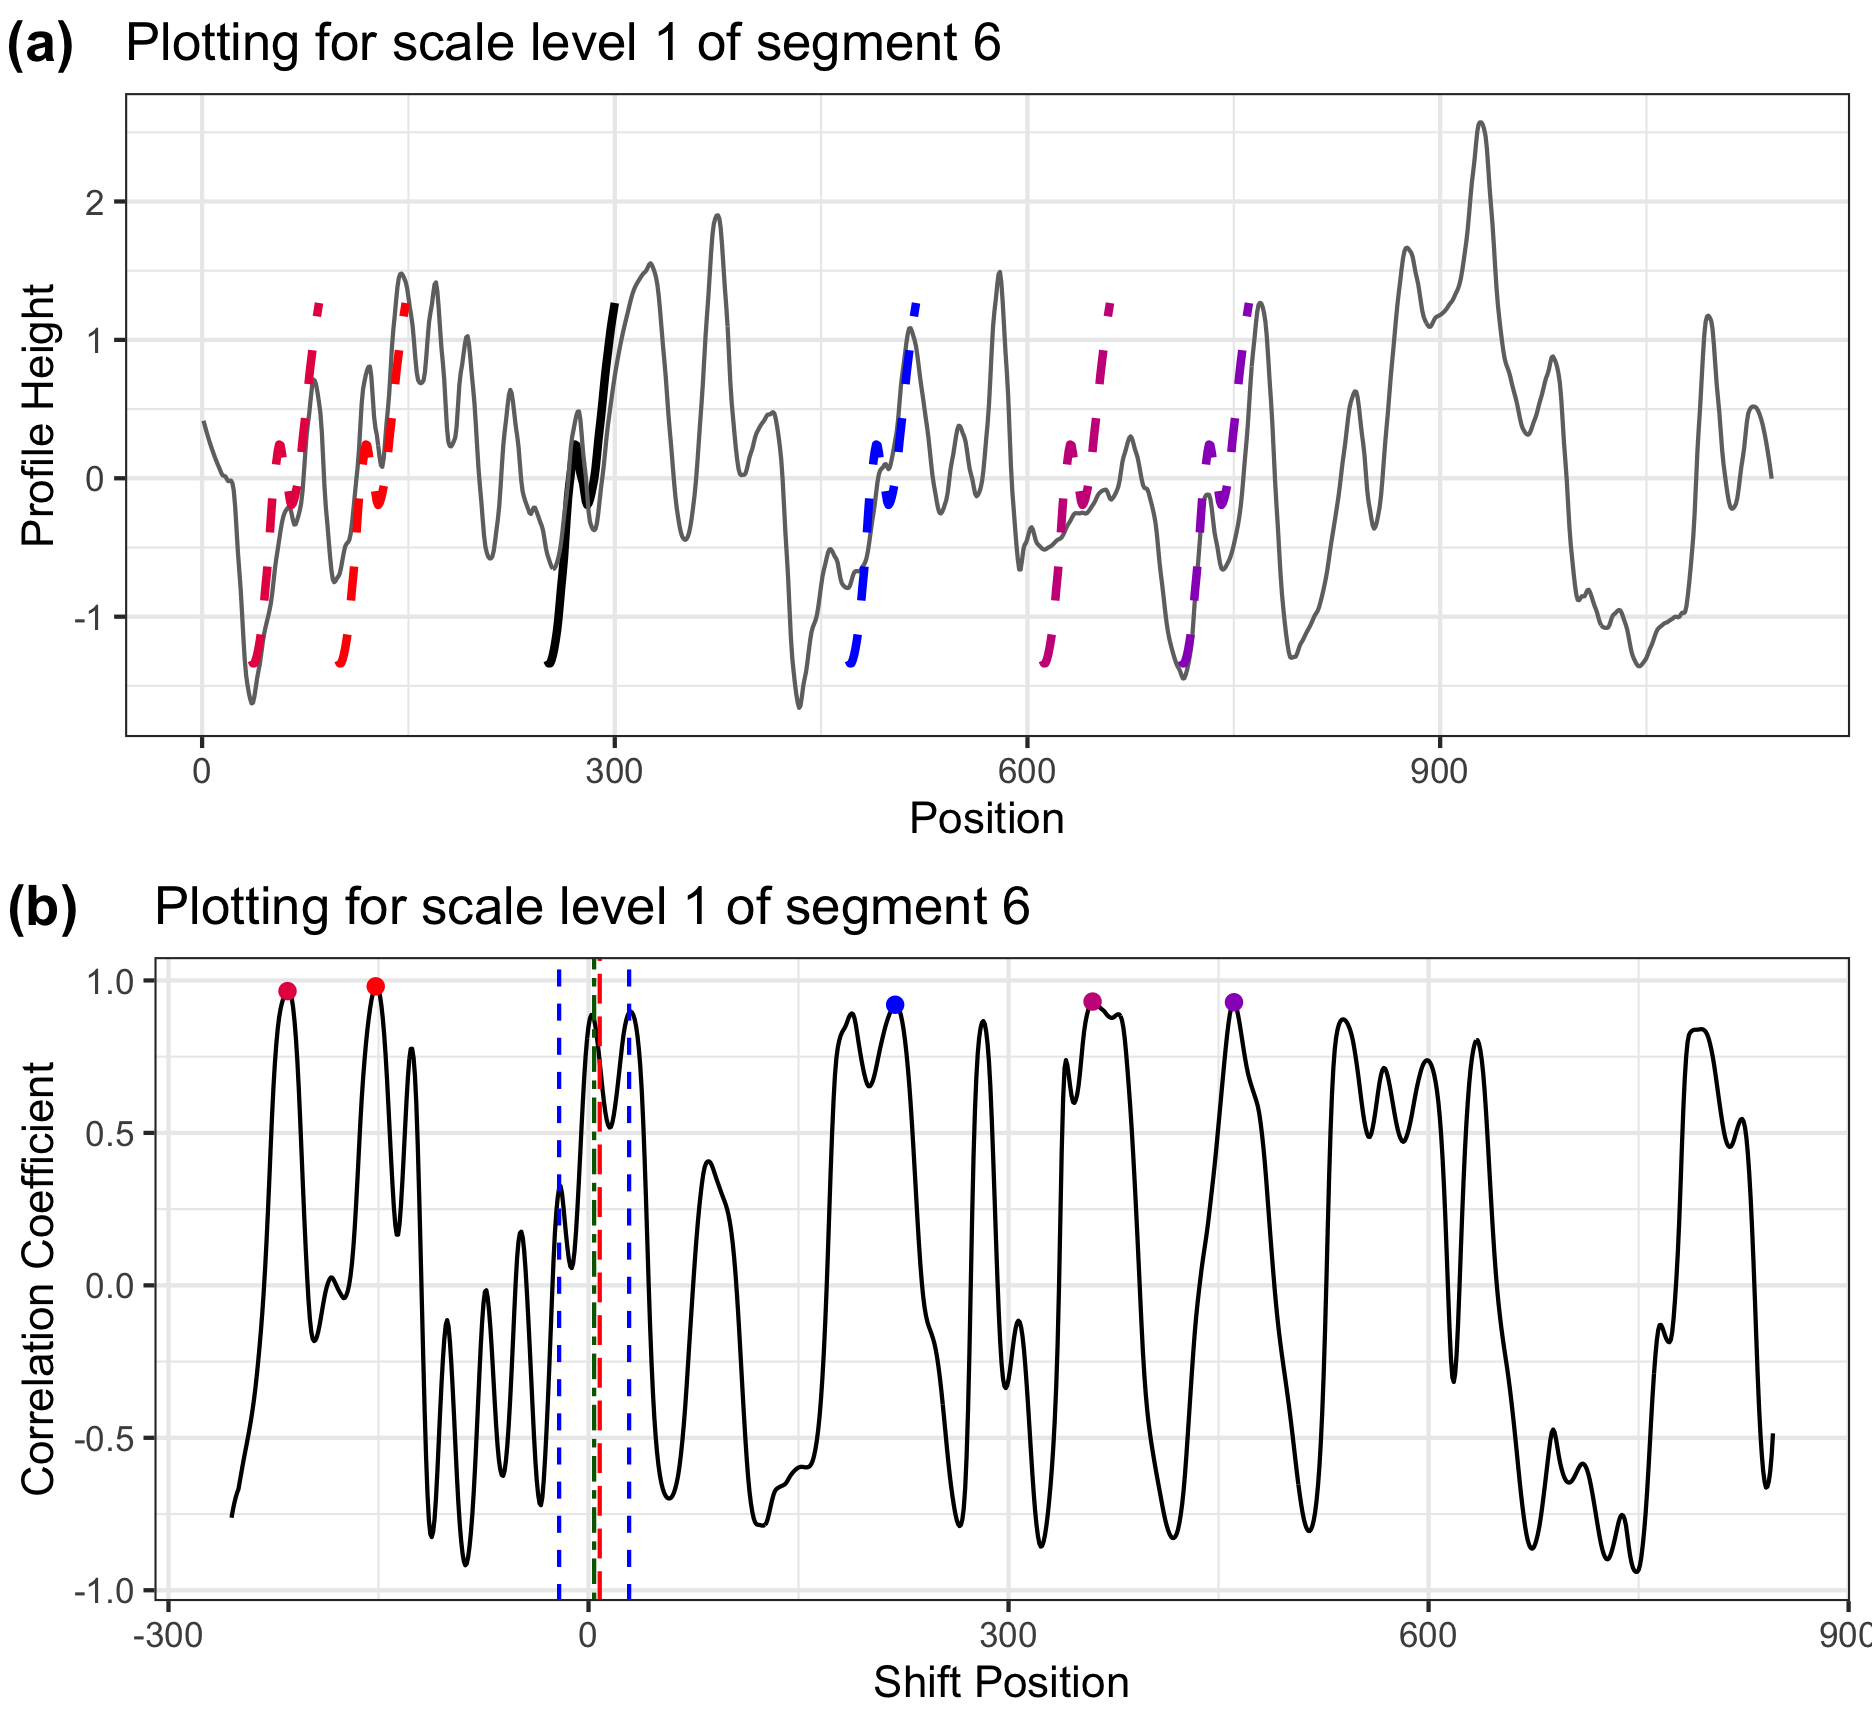
\includegraphics[width=.7\textwidth]{RJ-2022-035_files/figure-latex/segplots-web-1} 

}

\caption{Plot (a) shows segment\_plot for segment 6 at level one. The original position of segment 6 is indicated by the solid black line. Positions, where the segment achieves the 5 highest cross-correlations, are indicated by the dashed line segments. The scale\_ccf\_plot in plot (b) shows the cross-correlation curve between the reference signature and segment 6 at level one. The five highest peaks are marked by dots. The vertical red dashed line indicates the congruent registration position; the green dashed line shows a peak position in the highest segment level; the blue dashed lines show the tolerance zone around the green dashed line. We can see that none of the five highest peaks at level one falls within the tolerance zone, indicating that there is no consistent correlation peak or a candidate position identified by basis segment 6 under the multi-segment lengths strategy. Thus, the basis segment 6 doesn't vote for the congruent registration position and is not a cmps.}\label{fig:segplots-web}
\end{figure}

Additionally, users can have more insights about why segment 6 is not a congruent matching profile segment if we put the \texttt{segment\_plot} and \texttt{scale\_ccf\_plot} of all three segment levels together, as shown in Figure \ref{fig:segplots-all-web} with the help of \texttt{ggpubr::ggarrange()}.

\begin{verbatim}
library(ggpubr)

ggarrange(
  plotlist =
    unlist(seg_plot,
      recursive = FALSE
    ),
  ncol = 2,
  nrow = 3
)
\end{verbatim}

\begin{figure}

{\centering 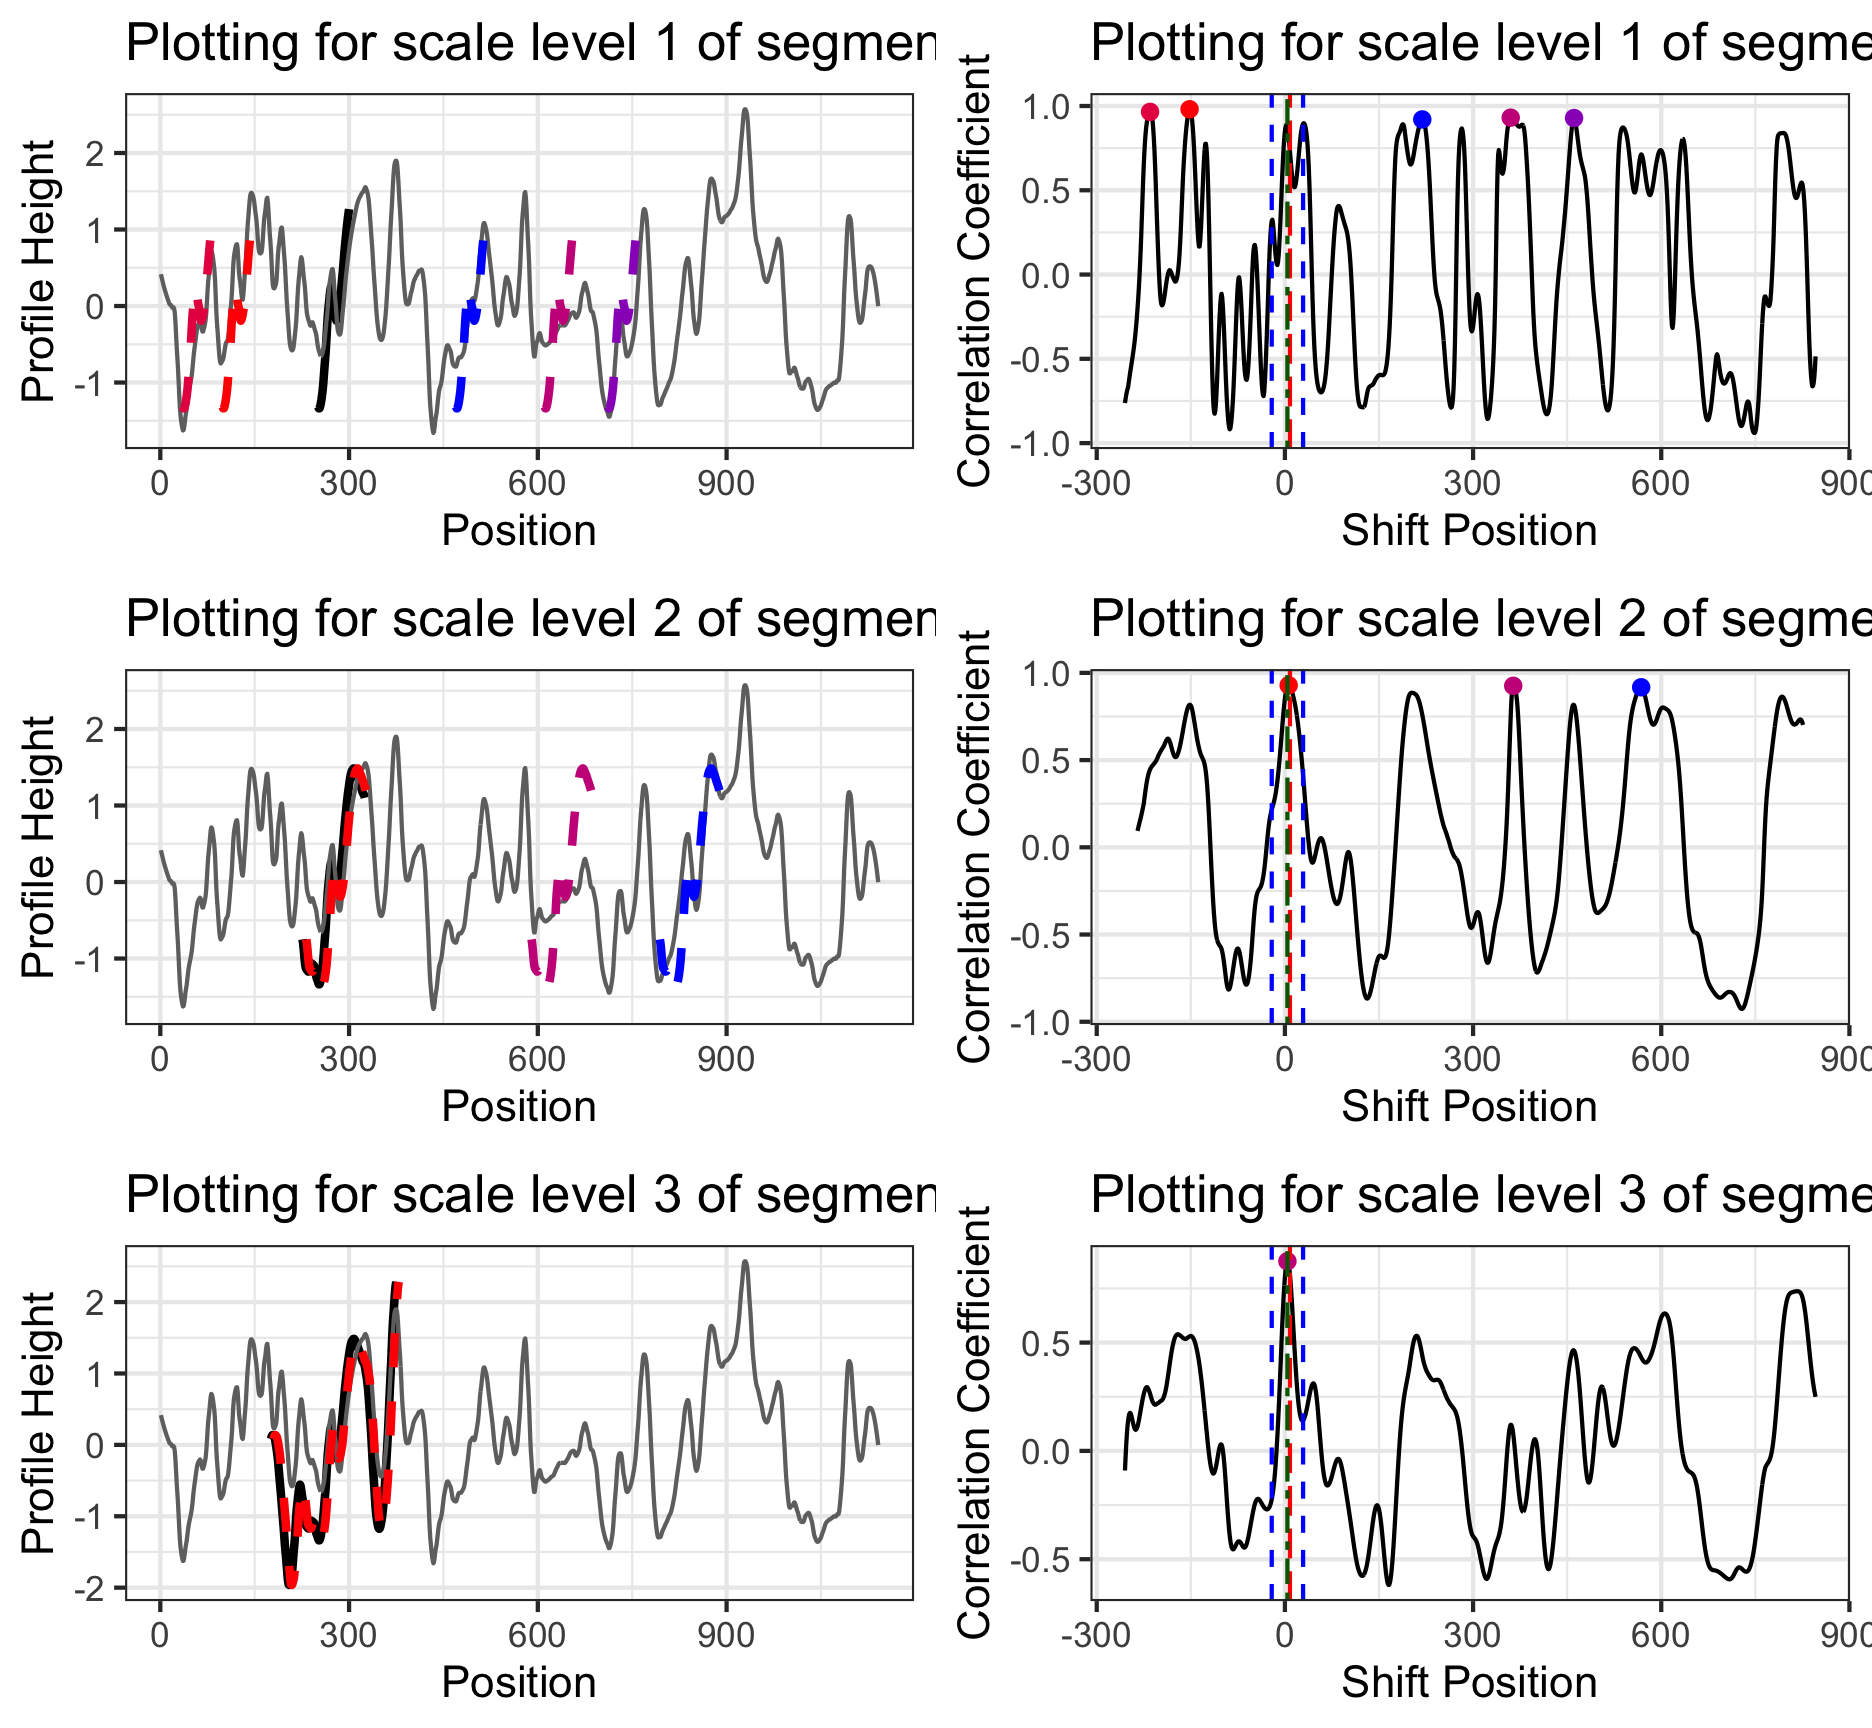
\includegraphics[width=.7\textwidth]{RJ-2022-035_files/figure-latex/segplots-all-web-1} 

}

\caption{Put segment\_plot and scale\_ccf\_plot of all three levels together. We are identifying the five highest peaks at level one, three peaks at level two, and one peak at level three since npeaks\_set = c(5, 3, 1). The highest peak position at level three is marked by the green dashed line across all segment levels. However, the highest peak on level three does not coincide with any of the top five highest peaks at level one. This indicates that there is no consistent correlation peak or a candidate position for basis segment 6 under the multi-segment lengths strategy.}\label{fig:segplots-all-web}
\end{figure}

In Figure \ref{fig:segplots-all-web}, the red vertical dashed line indicates the congruent registration position.
We can see that the basis segment 6 does obtain a peak near the congruent registration position at level two and level three, respectively; however, this position doesn't give one of the five highest peaks at level one.
As a result, segment 6 fails to identify the consistent correlation peak (ccp) and fails to become one of the congruent matching profile segments according to the multi-segment lengths strategy.
The identified top five peaks at level one are also examples of ``false positive'' peaks.
The ``true positive'' peak (the peak within the tolerance zone of the congruent registration position) is identified at level two and three by increasing the segment length, which justifies the usage of the multi-segment lengths strategy.

\hypertarget{evaluation-metrics}{%
\subsection{Evaluation metrics}\label{evaluation-metrics}}

\textbf{Metrics based on CMPS scores}

The CMPS algorithm measures the similarity between two signatures resulting in a similarity score of a land-to-level comparison.
Bullets fired from traditionally rifled barrels have multiple land and groove engraved areas.
Here, we are working with bullets fired from Ruger P85 barrels with six lands and grooves.
A comparison of two bullets, therefore, involves 36 land-to-land comparisons, resulting in 36 CMPS scores (as shown in Figure \ref{fig:tiles}).
In order to obtain a single similarity score of a bullet-level comparison, we need to summarize these 36 CMPS scores.
Two similarity metrics for bullet-level comparisons have been introduced in the literature (Chen et al. 2019): \(\mathrm{CMPS_{max}}\) and \(\mathrm{\overline{CMPS}_{max}}\).
\(\mathrm{CMPS_{max}}\) is the highest CMPS score obtained among all land-level comparisons, while \(\mathrm{\overline{CMPS}_{max}}\) is the highest possible mean CMPS score of land-level comparisons that are in the same phase:

In general, we assume each bullet has \(n\) land engravings (in our case \(n=6\)).
Let \(c_{ij}\) denote the CMPS score of a comparison between bullet 1 land \(i\) and bullet 2 land \(j\), for \(i,j = 1, \dots, n\).
Let \(\mathcal{P}_k\) denote bullet land pairs in phase \(k\) for \(k = 0, \dots, n-1\), and

\begin{align}
\mathcal{P}_k = \{ \left(i,j\right): i = 1, \dots, n ; \; j = \left(i + k\right) \;\mathrm{mod}\; n \}
\end{align}

, where \texttt{mod} denotes the modulo operation.
For example, \(\mathcal{P}_1 = \{ \left(1,2\right), \left(2,3\right), \left(3,4\right), \left(4,5\right), \left(5,6\right), \left(6,1\right) \}\) when \(n = 6\).
Let \(k^*\) denote the index of the highest phase.

With that, the two measures to evaluate accuracy used in Chen et al. (2019) are defined as

\begin{align}
\mathrm{CMPS_{max}} &= \max_{i,j} c_{ij} \text{ , and} \\
\mathrm{\overline{CMPS}_{max}} &= \frac{1}{n} \sum_{(i,j) \in \mathcal{P}_{k^*}} c_{ij} \text{ , where} \\
k^* &= \text{arg}\max\limits_{k} \left[  \frac{1}{n} \sum_{(i,j) \in \mathcal{P}_k} c_{ij}\right]
\end{align}

We can continue with the example used in previous sections.
\texttt{bullets} contains bullet signatures of two bullets, \texttt{bullet1} and \texttt{bullet2}.
As mentioned before, each bullet has six land engravings, resulting in six bullet signatures.
Thus, there are 36 pairwise bullet signature comparisons, resulting in 36 \(c_{ij}\) values in total.
We use multi-segment lengths strategy with default parameters to compute these CMPS scores, and the result is shown in Figure \ref{fig:tiles}.
We can see that in this example,

\[
\mathrm{CMPS_{max}} =  \max_{i,j} c_{ij} = 17
\]

and since bullet lands in phase \(\mathcal{P}_1\) gives the highest mean CMPS score (\(k^* = 1\)), we have

\[
\begin{aligned}
\mathrm{\overline{CMPS}_{max}} &= \frac{1}{6} \sum_{(i,j) \in \mathcal{P}_1} c_{ij} \\
                        &= \frac{1}{6} \left(c_{12} + c_{23} + c_{34} + c_{45} + c_{56} + c_{61}\right) \\
                        &= \frac{1}{6} \left(3+17+14+10+15+16\right) \\
                        &= 12.5
\end{aligned}
\]

\begin{figure}

{\centering 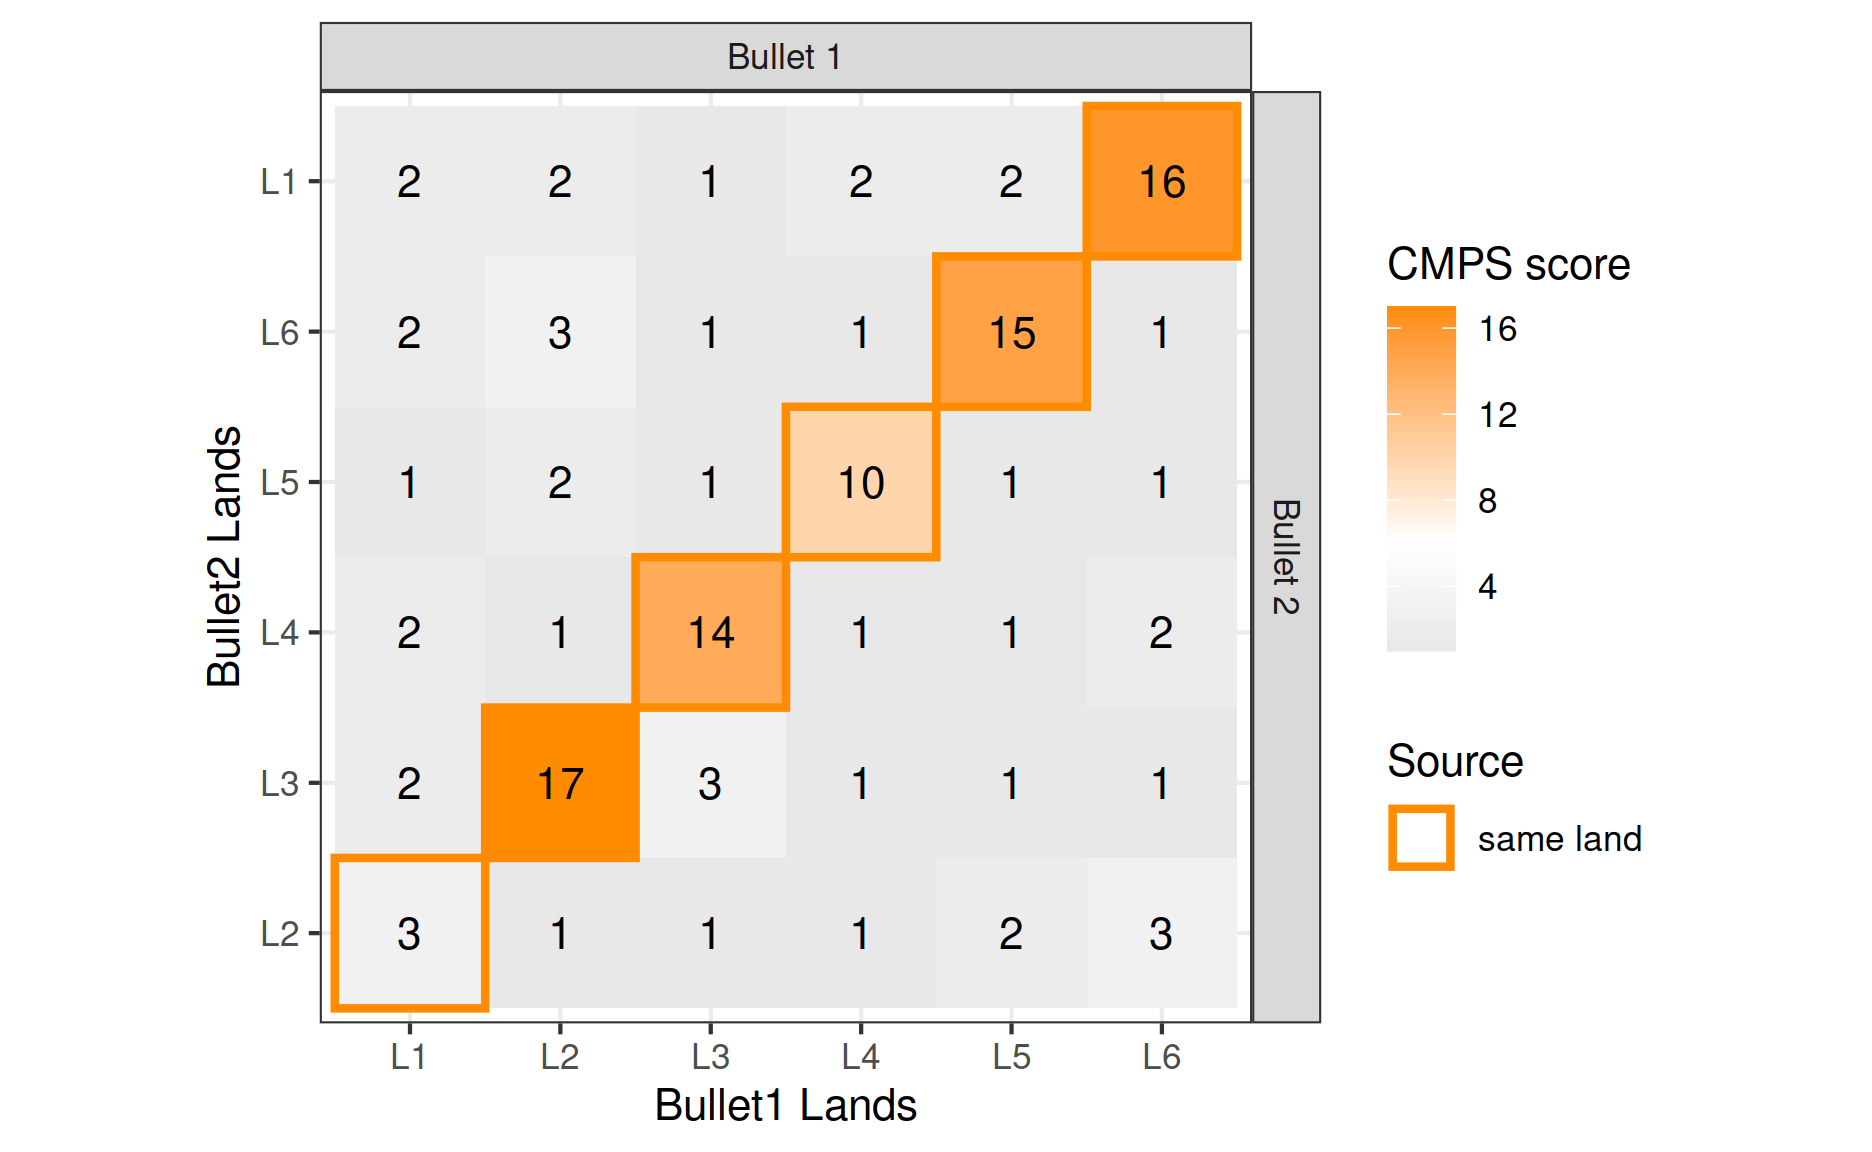
\includegraphics[width=.7\textwidth]{RJ-2022-035_files/figure-latex/tiles-1} 

}

\caption{CMPS scores of all 36 pairwise bullet signature comparisons for two bullets. Land engraving pairs generated by the same land (KM comparisons) are highlighted. Note that in this example the axis along Bullet 2 starts with Land 2. This corresponds to Phase 1 in equation (1).}\label{fig:tiles}
\end{figure}

However, both \(\mathrm{CMPS_{max}}\) and \(\mathrm{\overline{CMPS}_{max}}\) consider only relatively high CMPS scores and ignore the rest.
So we introduce a new metric based on CMPS scores called \(\mathrm{\overline{CMPS}_{diff}}\), which is the difference between \(\mathrm{\overline{CMPS}_{max}}\) and the mean of all other CMPS scores.
With our notation above, we have:

\begin{align}
\mathrm{\overline{CMPS}_{diff}} = \left[  \frac{1}{n} \sum_{(i,j) \in \mathcal{P}_{k^*}} c_{ij}\right] - \left[  \frac{1}{n\left(n-1\right)} \sum_{(i,j) \notin \mathcal{P}_{k^*}} c_{ij}\right]
\end{align}

\(\mathrm{\overline{CMPS}_{diff}}\) highlights the difference between CMPS scores of matching and non-matching comparisons.
If two bullets are non-matching, all 36 CMPS scores are expected to be small with relatively the same values, resulting in a \(\mathrm{\overline{CMPS}_{diff}}\) value close to 0.
For the example above, \(\mathrm{\overline{CMPS}_{diff}} = 12.5 - 1.53 = 10.97\)

\textbf{Scaled CMPS scores}

Another issue with the CMPS score is that the highest possible CMPS score (the total number of basis segments) might differ across comparisons (as shown in Figure \ref{fig:tiles2}(a)) due to different lengths of bullet signatures and different lengths of basis segments specified by the parameter.
A CMPS score of 5 might indicate a non-match if the highest possible CMPS score is 30 but indicate a match if the highest possible CMPS score is 6.
Thus, we introduce the scaled CMPS score, denoted as \(c^*_{ij}\).
Let \(s_{ij}\) denote the highest possible CMPS score or the total number of basis segments, then the scaled CMPS score \(c^*_{ij}\) is defined as the ratio of raw score and maximum score:

\begin{align}
c^*_{ij} = \frac{c_{ij}}{s_{ij}}
\end{align}

The scaled CMPS scores of the above example are shown in Figure \ref{fig:tiles2}(b).
Compared to the original CMPS scores, scaled scores have values within the interval \([0, 1]\) regardless of the length of the basis segments and therefore make a comparison of values possible across different parameter choices.
Similar to the original CMPS scores, we will denote the scaled CMPS scores adjusted for out-of-phase background values by \(\mathrm{\overline{CMPS^*}_{diff}}\).
For example, \(\mathrm{\overline{CMPS^*}_{diff}} = 0.498\) for Figure \ref{fig:tiles2}(b)

\begin{figure}

{\centering 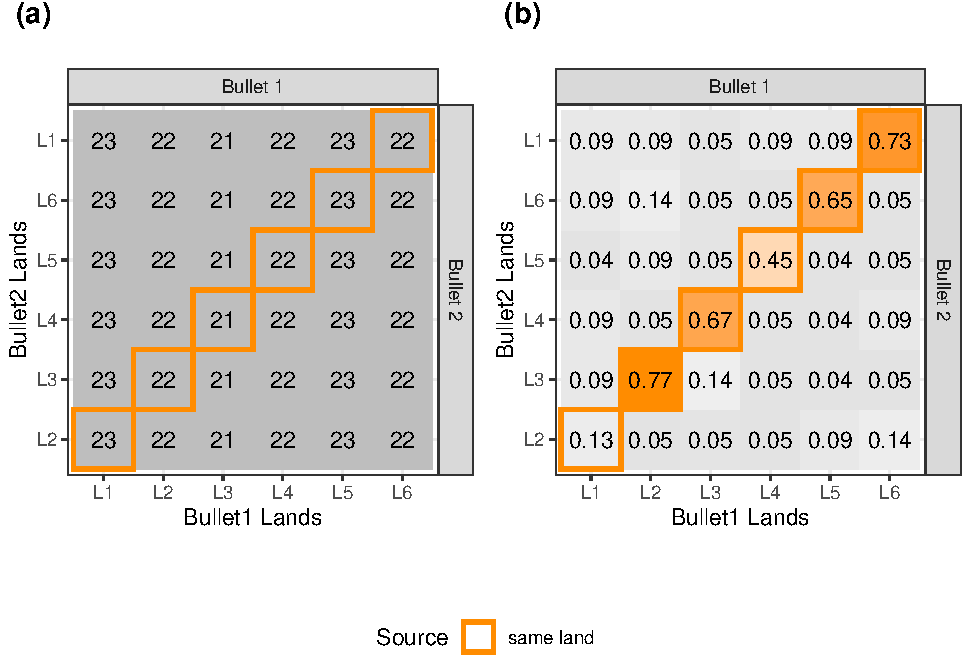
\includegraphics[width=.7\textwidth]{RJ-2022-035_files/figure-latex/tiles2-1} 

}

\caption{Plot (a) shows the highest possible CMPS scores (the total number of basis segments) for the 36 comparisons. (b) shows the scaled CMPS scores for the 36 comparisons.}\label{fig:tiles2}
\end{figure}

\textbf{Sum of squares ratio}

The ``sum of squares ratio'' quantifies how well two groups of values separate.
Let \(n_T\) denote the total number of observations, \(n_k\) denote the number of observations in group \(k\), and \(y_{kl}\) denote the \(l\)-th observation in group \(k\), for \(k = 1,2\) and \(l = 1, \dots, n_k\).
Let \(\bar{y}_{k.} = \frac{1}{n_k} \sum_{l=1}^{n_k} y_{kl}\) denote the mean value in group \(k\) and \(\bar{y}_{..} = \frac{1}{n_T} \left( \sum_{k} \sum_{l = 1}^{n_k} y_{kl} \right)\) denote the mean value of all observations.
Consider the following model:

\begin{align}
y_{kl} = \mu_k + e_{kl}
\end{align}

where \(\mu_k\) is the true mean of group \(k\) and \(e_{kl}\) is a random effect of different observations.
Then we can define the sum of squares ratio \(V\) as:

\begin{align}
V = \frac{\sum_k n_k \left(\bar{y}_{k.} - \bar{y}_{..} \right)^2}{\sum_k \sum_l^{n_k} \left(y_{kl} - \bar{y}_{k.} \right)^2 }.
\end{align}

The numerator of the sum of squares ratio \(V\) quantifies the variation between the two groups, while the denominator quantifies the variation within each group.
The sum of squares ratio \(V\) can be used as an index for evaluating scans, metrics, and different sets of parameters if the same data set is being used.
Some examples will be presented in the following section.
If we impose the normality and independence assumptions on the random effects \(e_{kl}\), the sum of squares ratio \(V\) becomes a scaled F-statistic with degrees of freedom of \(k-1\) and \(n_T - k\) and \(F = \frac{n_T - k}{k- 1} V\).
If we want to compare different data sets, stating that a certain setup can achieve better separation on one data set than another, we can scale the sum of squares ratio \(V\) and obtain the F-statistic and obtain the corresponding p-value as an index for comparison.

Using the sum of squares ratio \(V\) as an evaluation metric, we are able to construct a pipeline that aims to find the optimal parameter values for the CMPS algorithm by maximizing the sum of squares ratio.
Note that other measures of an algorithm, such as the accuracy and the AUC (Area Under the Curve), are also important and useful. But when algorithms achieve 100 percent accuracy and AUC value of 1, we need other measures such as the sum of squares ratio to further distinguish the performance of algorithms. In the following section, we will use the sum of squares ratio to compare the CMPS metrics introduced earlier and investigate the effects of different parameter settings.

\hypertarget{results}{%
\subsection{Results}\label{results}}

As presented in the work of Chen et al. (2019), researchers applied the CMPS method to scans of one of the Hamby sets.
While it is not explicitly stated in the paper, we presume this to be Hamby 252, as only those scans were publicly available at the time.
In order to show that our implementation of the CMPS algorithm is able to reproduce the results in Chen et al. (2019) and be used for other data sets, we applied our implementation to both Hamby set 252 and Hamby set 44.
Here we present how we obtained bullet signatures from the Hamby set data: for both Hamby 252 and Hamby 44, we started with scans in the form of x3p files in the database.
Following the framework proposed by Hare, Hofmann, and Carriquiry (2017), we used the same set of parameters, removed damaged bullet scans, obtained bullet signatures for each bullet land engraving, and removed outliers in bullet signatures.
Note that researchers of Chen et al. (2019) applied the CMPS algorithm to bullet signatures as well but used a framework different from ours.
However, since their work is not open-source, we were not able to follow their framework and were only able to reproduce the results for Hamby set 252 qualitatively.

\textbf{Hamby 252}

Figure \ref{fig:result1-252} shows the distribution of \(\mathrm{CMPS_{max}}\) and \(\mathrm{\overline{CMPS}_{max}}\) after we applied the CMPS algorithm to Hamby set 252 with the multi-segment lengths strategy.
The parameters we used in \texttt{extract\_feature\_cmps} for the CMPS algorithm are:

\begin{verbatim}
extract_feature_cmps(
  x, y,
  seg_length = 50,
  Tx = 25,
  npeaks_set = c(5, 3, 1),
  include = "nseg"
)
\end{verbatim}

As noted above, the CMPS scores we found here are not exactly the same as those presented in Chen et al. (2019) since we were not able to follow their framework, but the results presented in Figure \ref{fig:result1-252} are qualitatively equivalent to those presented in Chen et al. (2019), showing a clear separation between scores based on comparisons from known matches (KM) and scores from comparisons of known non-matches (KNM) for both \(\mathrm{CMPS_{max}}\) and \(\mathrm{\overline{CMPS}_{max}}\).

Additionally, to mimic the parameters used in Chen et al. (2019), we set \texttt{seg\_length\ =\ 50} and \texttt{Tx\ =\ 25} to make sure that each basis segment has a length of 78.125 \textmu m and the tolerance zone is \(\pm 39.0625\) \textmu m (one unit represents 1.5625 \textmu m for Hamby set 252).

The sum of squares ratios are 20.64 and 28.96 for \(\mathrm{CMPS_{max}}\) and \(\mathrm{\overline{CMPS}_{max}}\), respectively.
This indicates that even though scores from \(\mathrm{CMPS_{max}}\) for known-match comparisons are larger than scores from the averaged version of \(\mathrm{\overline{CMPS}_{max}}\), these scores achieve a better separation between the two groups of comparisons.

\begin{figure}

{\centering 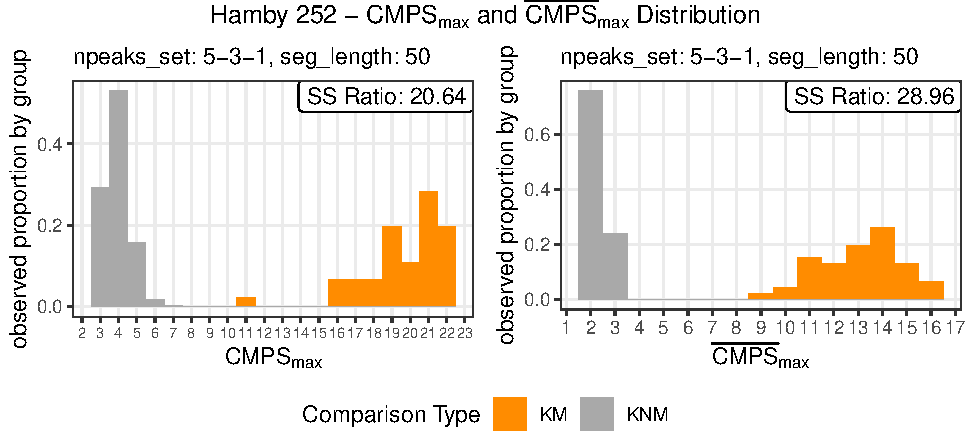
\includegraphics[width=400px]{RJ-2022-035_files/figure-latex/result1-252-1} 

}

\caption{Distribution of $\mathrm{CMPS_{max}}$ and $\mathrm{\overline{CMPS}_{max}}$ for Hamby 252; outliers are removed in bullet signatures; seg\_length = 50, Tx = 25, npeaks\_set = c(5,3,1); instead of showing the counts on the y-axis, we present the observed proportions conditioned on KM group and KNM group to enhance the visibility of the bars. }\label{fig:result1-252}
\end{figure}

\textbf{Hamby 44}

Similar procedures are applied to Hamby set 44, and Figure \ref{fig:result1-44} shows the distribution of \(\mathrm{CMPS_{max}}\) and \(\mathrm{\overline{CMPS}_{max}}\), respectively.
The parameters used in \texttt{extract\_feature\_cmps} are:

\begin{verbatim}
extract_feature_cmps(
  x, y,
  seg_length = 61,
  Tx = 30,
  npeaks_set = c(5, 3, 1),
  include = "nseg"
)
\end{verbatim}

Since the resolution of Hamby 44 is set to 1.29 \textmu m per unit, we make \texttt{seg\_length\ =\ 61} and \texttt{Tx\ =\ 30} to ensure that the setup of Hamby set 44 is similar to that of Hamby set 252, resulting in basis segments of 78.69 \textmu m and the tolerance zone of \(\pm 38.7\) \textmu m.

As shown in Figure \ref{fig:result1-44}, again, we are able to see a clear separation between the known match comparisons and the known non-match comparisons, even though the separation is relatively small compared with that of Hamby set 252, which is also indicated by the sum of squares ratios.
For this specific set of parameters, the sum of squares ratios are 8.87 and 10.64 for \(\mathrm{CMPS_{max}}\) and \(\mathrm{\overline{CMPS}_{max}}\), respectively.
This might suggest that we could enlarge the separation in terms of the sum of squares ratio by using other CMPS metrics and other sets of parameters.

\begin{figure}

{\centering 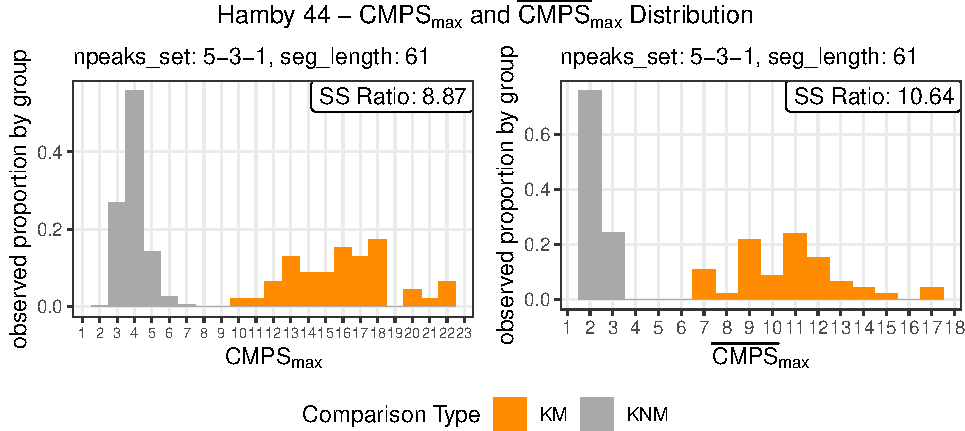
\includegraphics[width=400px]{RJ-2022-035_files/figure-latex/result1-44-1} 

}

\caption{Distribution of $\mathrm{CMPS_{max}}$ and $\mathrm{\overline{CMPS}_{max}}$ for Hamby 44; outliers are removed in bullet signatures; seg\_length = 61, Tx = 30, npeaks\_set = c(5,3,1); instead of showing the counts on the y-axis, we present the observed proportions conditioned on KM group and KNM group to enhance the visibility of the bars. }\label{fig:result1-44}
\end{figure}

\textbf{Comparing CMPS metrics and parameters}

\begin{figure}

{\centering 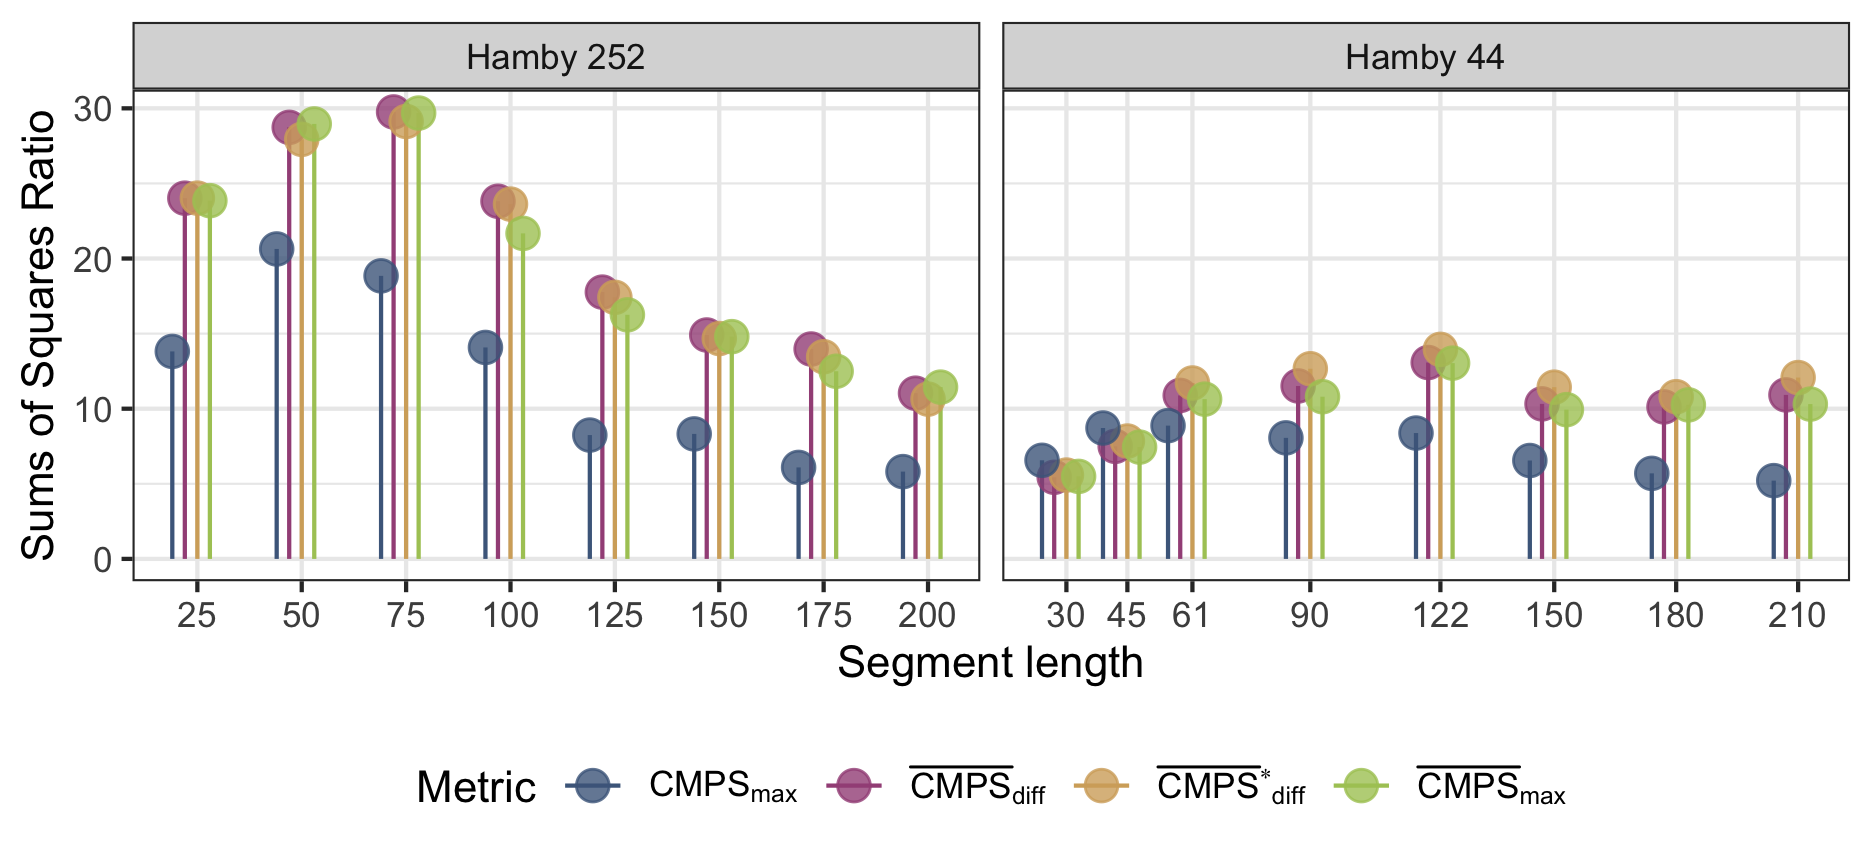
\includegraphics[width=400px]{RJ-2022-035_files/figure-latex/param-seg-plot-1} 

}

\caption{Comparison of results from the CMPS algorithm based on different basis segment lengths (parameter seg\_length). Only the $\mathrm{CMPS_{max}}$ metric suggests that the default values for the basis segment length result in the best separation. Better separation is achieved based on the modified CMPS metrics, including the newly suggested ones. For Hamby 252 these metrics agree on a segment length of 75, and a segment length of 122 for Hamby 44 yields better results. }\label{fig:param-seg-plot}
\end{figure}

\begin{figure}

{\centering 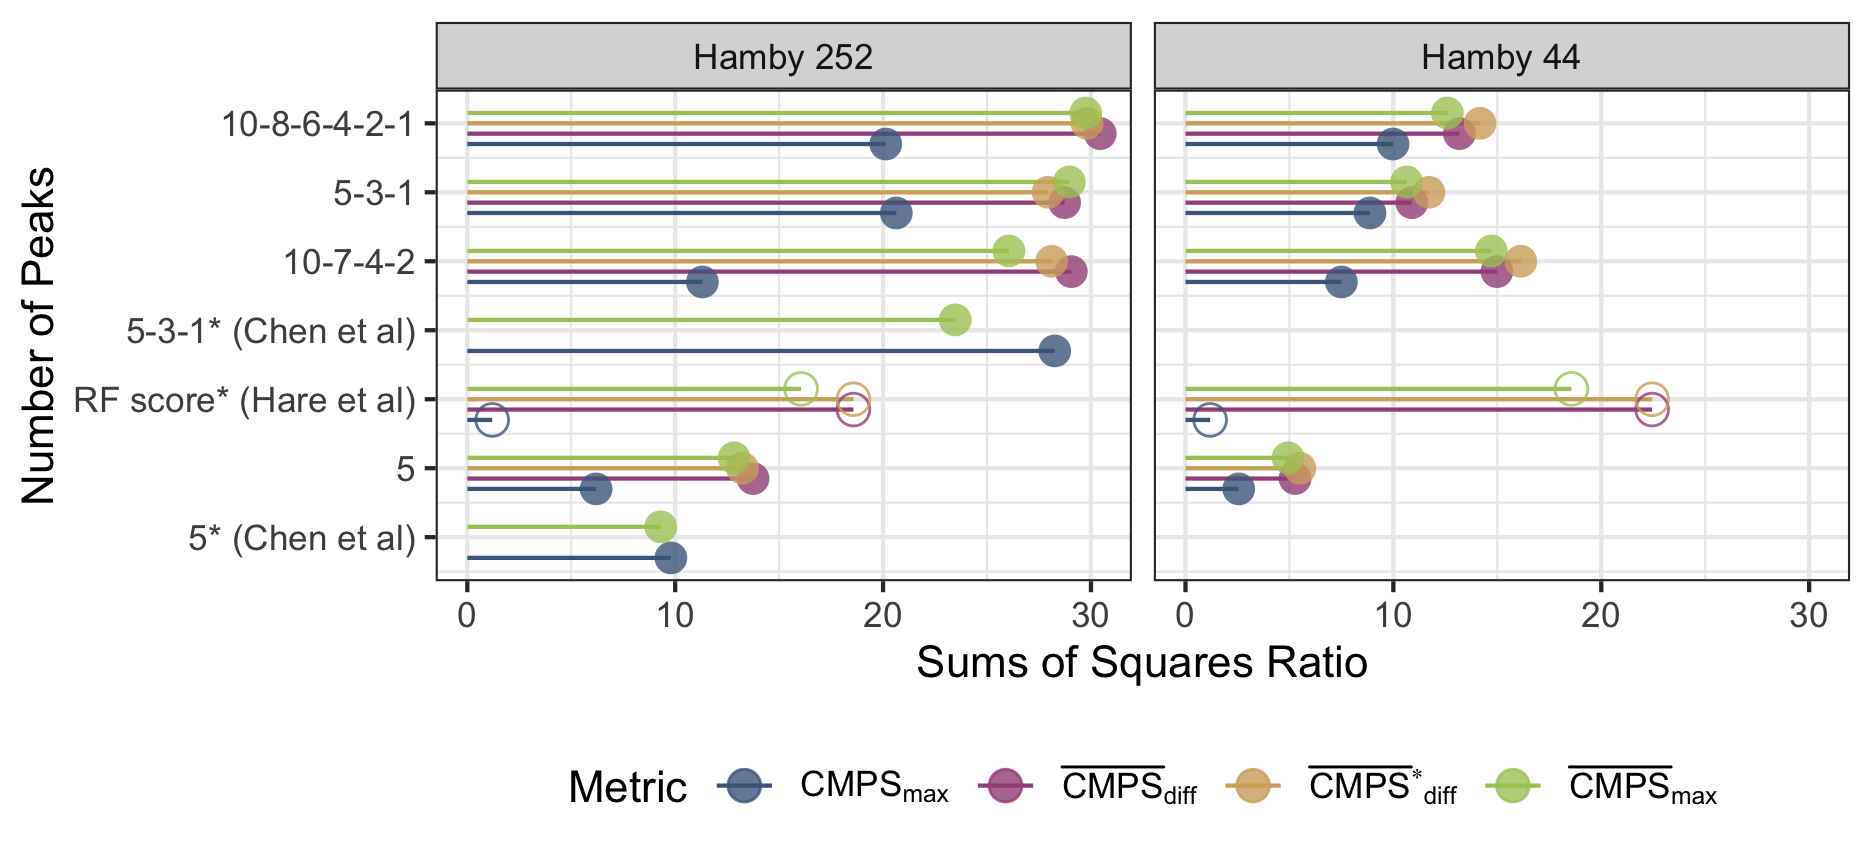
\includegraphics[width=400px]{RJ-2022-035_files/figure-latex/param-npeak-plot-1} 

}

\caption{Comparison of CMPS results based on different strategies of number of peak selections. Starred results compare CMPS performance with results published in the literature. Results for the random forest score are represented with circles because the metrics are computed not based on the CMPS scores, but on the random forest scores with the same logic. Since random forest scores lie within the interval $[0, 1]$, scaling the random forest scores will not change the results.}\label{fig:param-npeak-plot}
\end{figure}

We investigated the effects of different sets of parameters in the example of both Hamby sets 252 and 44.
More specifically, we investigated the separation achieved using the \pkg{cmpsR} implementation under various segment lengths (controlled by the parameter \texttt{seg\_length}). Specifically, we fixed the parameter \texttt{npeaks\_set} that controls the number of peaks at each segment level to be \texttt{npeaks\_set\ =\ c(5,\ 3,\ 1)} and modified the parameter \texttt{seg\_length}.
Figure \ref{fig:param-seg-plot} shows that the default values of \texttt{seg\_length} for Hamby 252 and Hamby 44 (50 for Hamby 252 and 61 for Hamby 44, which represent 78.125 \textmu m and 78.69 \textmu m, respectively) result in high values of the sum of squares ratio, no matter which CMPS metrics are used for an evaluation.
However, we also see, that for Hamby set 252 a basis segment length of 75 is a better choice than the default segment length; a basis segment length of 122 results in a higher value of the sum of squares ratio for Hamby 44.

Figure \ref{fig:param-npeak-plot} shows the results of the CMPS algorithm using different strategies for identifying peaks in the correlation structure between signatures. Basis segment length is fixed to the default level for this evaluation.
As can be seen in Figure \ref{fig:param-npeak-plot}, the default value of \texttt{npeaks\_set} (\texttt{npeaks\_set\ =\ c(5,\ 3,\ 1)}) leads to promising results in terms of the sum of squares ratio; however, other choices of \texttt{npeaks\_set} match and exceed this sum of squares ratio value.

As seen before, the results suggest that the \(\mathrm{CMPS_{max}}\) metric produces the least amount of separation compared with the other three CMPS metrics.
They also suggest that the two newly proposed metrics, \(\mathrm{\overline{CMPS}_{diff}}\) and \(\mathrm{\overline{CMPS^*}_{diff}}\), lead to equally good or even better results as \(\mathrm{\overline{CMPS}_{max}}\).
Because \(\mathrm{\overline{CMPS^*}_{diff}}\) relies on a scaled version of CMPS scores, it is more comparable to other similarity scores and summarizes the out-of-phase background CMPS scores, making it superior to the other CMPS metrics.

What we can also observe in Figure \ref{fig:param-seg-plot} and Figure \ref{fig:param-npeak-plot} is that the values of the sum of squares ratio for Hamby 44 is lower than those for Hamby 252.
This might be because determining the source is a harder task for Hamby 44 than for Hamby 252, but also suggests that the choice of parameters also depends on the resolution or the scanning process of the data set.
The same set of parameters might work for one data set, but not work equally well for another.

The purpose of the results shown in Figure \ref{fig:param-seg-plot} and Figure \ref{fig:param-npeak-plot} is not to determine the ``best'' parameters for the CMPS algorithm, but to show that the sum of squares ratio can be used as an evaluation measure to compare different parameters, metrics, or scans.
A pipeline that maximizes the sum of squares ratio might help researchers determine the set of parameters that work best for their data.
But a large database that is representative is what we really need in order to fully understand and cross-validate the parameters of the CMPS algorithm.

\textbf{Comparing with original results and the random forest model}

Chen et al. (2019) present histograms of \(\mathrm{CMPS_{max}}\) and \(\mathrm{\overline{CMPS}_{max}}\) for \texttt{npeaks\_set\ =\ 5} and \texttt{npeaks\_set\ =\ c(5,\ 3,\ 1)} with (presumably) Hamby 252.
The values in these histograms allow us to calculate the sum of squares ratios and include the results in Figure \ref{fig:param-npeak-plot} as well.
They are marked by an asterisk at the top right corner in Figure \ref{fig:param-npeak-plot}.
The sum of squares ratios we obtained for \texttt{npeaks\_set\ =\ 5} and \texttt{npeaks\_set\ =\ c(5,\ 3,\ 1)} is slightly higher than those obtained from the histograms of Chen et al. (2019).
It's curious to see that for the Hamby 252 results published in Chen et al. (2019) the \(\mathrm{{CMPS}_{max}}\) metric achieves values of the sum of squares ratio higher than those achieved by the \(\mathrm{\overline{CMPS}_{max}}\) metric.

Since the researchers of Chen et al. (2019) did not use \(\mathrm{\overline{CMPS}_{diff}}\) or \(\mathrm{\overline{CMPS^*}_{diff}}\), and they did not apply the CMPS algorithm to the Hamby set 44, we were not able to compare those results.

In Figure \ref{fig:param-npeak-plot}, we also included the sum of squares ratios computed from the random forest scores (Hare, Hofmann, and Carriquiry 2017) for different metrics.
The random forest model presented in Hare, Hofmann, and Carriquiry (2017) was trained at the Center for Statistics and Applications in Forensic Evidence (CSAFE) and is publicly available in the R package \texttt{bulletxtrctr} (Hofmann, Vanderplas, and Krishnan 2019).
Similar to the CMPS algorithm, this random forest model produces a score to quantify the similarity of a land-by-land comparison.
The RF scores lie in an interval of {[}0,1{]} making them most comparable to the scaled CMPS scores.
We applied the logic of \(\mathrm{{CMPS}_{max}}\), \(\mathrm{\overline{CMPS}_{max}}\), and \(\mathrm{\overline{CMPS}_{diff}}\) to the random forest scores and obtained results of the random forest model for different metrics.
As shown in Figure \ref{fig:param-npeak-plot}, the random forest model does not achieve the sum of squares ratio as high as those achieved by the top CMPS algorithms for Hamby 252, but it does achieve better results for Hamby 44.
This might suggest that inclusion of the CMPS score as an additional feature in the random forest model training might be beneficial for an overall separation to determine the source.

For details about the implementation, examples, and results, please refer to the ``Supplementary materials''.

\hypertarget{conclusion}{%
\subsection{Conclusion}\label{conclusion}}

In this paper, we present the \pkg{cmpsR} package, an open-source implementation of the Congruent Matching Profile Segments (CMPS) algorithm (Chen et al. 2019), and apply it to two datasets in Hamby study (Hamby, Brundage, and Thorpe 2009) to show its potential for further research.
The CMPS algorithm was proposed by NIST in 2019 and was made for objective tool marks comparisons.
We introduce the basic logic of the CMPS algorithm and layout its implementation in the \pkg{cmpsR} package.
We also showcase the functionality of the \pkg{cmpsR} package with a small dataset example that is included in the package.
In the \pkg{cmpsR} package we implement some graphing tools for users to visualize results and to gain a better understanding of both the algorithm and the results.

Additionally, we propose two new metrics based on the CMPS scores and compare the new metrics with the existing metrics.
We also introduce a principled evaluation framework of algorithmic results using a measure based on the sum of squares ratio.
We showcase the implementation with two datasets in the Hamby study (Hamby set 252 and Hamby set 44) and compare the CMPS algorithm using different sets of parameters and different metrics, following the evaluation framework based on the sum of squares ratio.
The results obtained are promising: we were both able to reproduce the results in Chen et al. (2019) qualitatively and achieve a clear separation between the known match (KM) comparisons and known non-match (KNM) comparisons in another bullet study.
However, the comparisons among different sets of parameters suggest that the optimal choice for parameter settings varies between different datasets.

Note, that the main difference between Hamby sets 44 and 252 is that they were taken with different resolution scanning devices. The bullets for Hamby 44 and Hamby 252 are fired from the same ten consecutively rifled P-85 Ruger barrels. The difference in parameter settings for optimal differentiation between same-source comparisons and different-source comparisons is therefore quite surprising. In the next steps, we need validation studies similar to Vanderplas et al. (2020) - trying out the CMPS algorithm on different firearms and ammunition combinations to test the limits of the algorithm. The evaluation framework we proposed based on the sum of squares ratio will facilitate such studies and other validation of the algorithm.

Comparisons of the R implementation of the CMPS algorithm with the random forest model proposed by Hare, Hofmann, and Carriquiry (2017) suggest that adding the CMPS score as an additional feature in the random forest model might add further separation between known match (KM) comparisons and known non-match (KNM) comparisons.

The open-source implementation of the CMPS algorithm provided by the \pkg{cmpsR} package is just one step towards to the framework of open science. Open science is particularly important to fields like forensic science where transparency and accuracy are critical to fair justice.
Open-source implementations not only allow a peer-review but also facilitate further research, such as parameter cross-validations, method comparisons, and the development of statistical methods for modeling KM and KNM CMPS score distributions, which can then be used for error-rate estimations and fair applications that were called for by the PCAST (President's Council of Advisors on Science and Technology 2016) report.
However, having open-source implementations is not enough for open science.
In order to actually build the world of open science, many other efforts, such as open evaluation, open access publication, open educational resources, etc., are still needed.
The database built and maintained by the National Institute of Standards and Technology is a good example of open data.
What we are aiming for is an open system that is able to collect open results, compare multiple algorithms using multiple datasets, and evaluate algorithmic variation and accuracy.
The evaluation metric we proposed in this paper can be used to compare different algorithms or even different datasets and is a snippet of this open system.
But the core of this open system is the open science culture and contributions of the community.

\hypertarget{acknowledgement}{%
\subsection{Acknowledgement}\label{acknowledgement}}

This work was funded (or partially funded) by the Center for Statistics and Applications in Forensic Evidence (CSAFE) through Cooperative Agreements 70NANB15H176 and 70NANB20H019 between NIST and Iowa State University, which includes activities carried out at Carnegie Mellon University, Duke University, University of California Irvine, University of Virginia, West Virginia University, University of Pennsylvania, Swarthmore College and University of Nebraska, Lincoln.

\hypertarget{supplementary-materials}{%
\subsection{Supplementary materials}\label{supplementary-materials}}

The zip file ``supplementary-files.zip'' contains R scripts for reproducing all aspects of this paper.

\textbf{Data not included in ``supplementary-files.zip''}

The processed data of Hamby set 252 and Hamby set 44 are stored in two \texttt{.rds} files:

\begin{itemize}
\tightlist
\item
  \href{https://github.com/willju-wangqian/CMPSpaper/blob/main/reproducible/bullet_signatures_etc/BulletSignatures252.rds}{\texttt{BulletSignatures252.rds}}
\item
  \href{https://github.com/willju-wangqian/CMPSpaper/blob/main/reproducible/bullet_signatures_etc/BulletSignatures44.rds}{\texttt{BulletSignatures44.rds}}
\end{itemize}

And the ground truth of Hamby set 252 is provided in \href{https://github.com/willju-wangqian/CMPSpaper/blob/main/reproducible/bullet_signatures_etc/StudyInfo.xlsx}{\texttt{StudyInfo.xlsx}}

Due to the size of the file, these processed data are not included in the ``supplementary-files.zip'', but the links are provided for download.

In order to reproduce the results in the paper, please download ``BulletSignatures252.rds'', ``BulletSignatures44.rds'', and ``StudyInfo.xlsx'' and save them in a folder named ``bullet\_signatures\_etc''. And place the folder ``bullet\_signatures\_etc'' into the folder of all the R scripts of ``supplementary-files.zip''.

Please check out the folder structure of \href{https://github.com/willju-wangqian/CMPSpaper/tree/main/reproducible}{the \texttt{reproducible} folder} for reference.

\textbf{File description}

\begin{itemize}
\tightlist
\item
  \texttt{hamby*\_result\_generator.R}: these R scripts take the processed data of Hamby set 252 and Hamby set 44, generate preliminary results used in the paper, and save the results in the \texttt{.csv} format in the folder \texttt{data-csv}. Please make sure that the package versions of \texttt{bulletxtrctr} and \texttt{cmpsR} meet the requirements.
\item
  \texttt{rds\_generator.R}: this R script takes the generated \texttt{.csv} files and produce \texttt{CMPSpaper\_results.rds}. \texttt{CMPSpaper\_results.rds} is identical to \texttt{data/CMPSpaper\_results.rds} and is used generate figures and other results presented in the paper.
\end{itemize}

\textbf{Data included in ``supplementary-files.zip''}

\begin{itemize}
\tightlist
\item
  \texttt{data-csv}: this folder contains \texttt{.csv} files we generated using R scripts \texttt{hamby*\_result\_generator.R}
\item
  \texttt{CMPSpaper\_results.rds}: this is the \texttt{.rds} file we generated using R script \texttt{rds\_generator.R}
\end{itemize}

These data can be used as reference or example results of the reproducible codes

\begin{itemize}
\tightlist
\item
  \texttt{csafe\_rf2.rds}: this \texttt{.rds} file contains the random forest model used in this paper
\end{itemize}

\hypertarget{references}{%
\section*{References}\label{references}}
\addcontentsline{toc}{section}{References}

\hypertarget{refs}{}
\begin{CSLReferences}{1}{0}
\leavevmode\vadjust pre{\hypertarget{ref-afte}{}}%
AFTE Criteria for Identification Committee. 1992. {``Theory of Identification, Range Striae Comparison Reports and Modified Glossary Definitions.''} \emph{AFTE Journal} 24 (3): 336--40.

\leavevmode\vadjust pre{\hypertarget{ref-brundage}{}}%
Brundage, David J. 1998. {``{The Identification of Consecutively Rifled Gun Barrels}.''} \emph{AFTE Journal} 30 (3): 438--44.

\leavevmode\vadjust pre{\hypertarget{ref-shiny}{}}%
Chang, Winston, Joe Cheng, JJ Allaire, Carson Sievert, Barret Schloerke, Yihui Xie, Jeff Allen, Jonathan McPherson, Alan Dipert, and Barbara Borges. 2021. \emph{{shiny: Web Application Framework for R}}. \url{https://CRAN.R-project.org/package=shiny}.

\leavevmode\vadjust pre{\hypertarget{ref-cmps}{}}%
Chen, Zhe, Wei Chu, Johannes A. Soons, Robert M. Thompson, John Song, and Xuezeng Zhao. 2019. {``{Fired bullet signature correlation using the Congruent Matching Profile Segments (CMPS) method}.''} \emph{Forensic Science International} 305: Article 109964, (10 pages). https://doi.org/\url{https://doi.org/10.1016/j.forsciint.2019.109964}.

\leavevmode\vadjust pre{\hypertarget{ref-ChumbleyL_Scott2010VoTM}{}}%
Chumbley, L. Scott, Max D Morris, M. James Kreiser, Charles Fisher, Jeremy Craft, Lawrence J Genalo, Stephen Davis, David Faden, and Julie Kidd. 2010. {``Validation of Tool Mark Comparisons Obtained Using a Quantitative, Comparative, Statistical Algorithm: VALIDATION OF TOOL MARK COMPARISONS.''} \emph{Journal of Forensic Sciences} 55 (4): 953--61. https://doi.org/\url{https://doi.org/10.1111/j.1556-4029.2010.01424.x}.

\leavevmode\vadjust pre{\hypertarget{ref-loess}{}}%
Cleveland, William S., Eric Grosse, and William M. Shyu. 1991. {``Local Regression Models.''} In \emph{Statistical Models in s}, edited by John M. Chambers and Tibshirani J. Hastie, 309--76. Boca Raton, Florida: Chapman; Hall/CRC.

\leavevmode\vadjust pre{\hypertarget{ref-nrc}{}}%
Committee on Identifying the Needs of the Forensic Sciences of the National Research Council. 2009. {``{Strengthening Forensic Science in the United States: A Path Forward}.''} \url{https://www.ncjrs.gov/pdffiles1/nij/grants/228091.pdf}; National Academies Press.

\leavevmode\vadjust pre{\hypertarget{ref-Hamby:2019}{}}%
Hamby, James E., David J. Brundage, Nicholas D. K. Petraco, and James W. Thorpe. 2019. {``A {Worldwide} {Study} of {Bullets} {Fired} {From} 10 {Consecutively} {Rifled} {9mm} {RUGER} {Pistol} {Barrels}---{Analysis} of {Examiner} {Error} {Rate}.''} \emph{Journal of Forensic Sciences} 64 (2): 551--57. \url{https://doi.org/10.1111/1556-4029.13916}.

\leavevmode\vadjust pre{\hypertarget{ref-hamby}{}}%
Hamby, James E., David J. Brundage, and James W. Thorpe. 2009. {``{The Identification of Bullets Fired from 10 Consecutively Rifled 9mm Ruger Pistol Barrels: A Research Project Involving 507 Participants from 20 Countries}.''} \emph{AFTE Journal} 41 (2): 99--110.

\leavevmode\vadjust pre{\hypertarget{ref-aoas}{}}%
Hare, Eric, Heike Hofmann, and Alicia Carriquiry. 2017. {``Automatic Matching of Bullet Land Impressions.''} \emph{Ann. Appl. Stat.} 11 (4): 2332--56. \url{https://doi.org/10.1214/17-AOAS1080}.

\leavevmode\vadjust pre{\hypertarget{ref-bulletxtrctr}{}}%
Hofmann, Heike, Susan Vanderplas, and Ganesh Krishnan. 2019. \emph{Bulletxtrctr: Automatic Matching of Bullet Striae}. \url{https://heike.github.io/bulletxtrctr/}.

\leavevmode\vadjust pre{\hypertarget{ref-x3ptools}{}}%
Hofmann, Heike, Susan Vanderplas, Ganesh Krishnan, and Eric Hare. 2020. \emph{{x3ptools: Tools for Working with 3D Surface Measurements}}. \url{https://github.com/heike/x3ptools}.

\leavevmode\vadjust pre{\hypertarget{ref-pmid30444940}{}}%
Krishnan, G., and H. Hofmann. 2019. {``{{A}dapting the {C}humbley {S}core to {M}atch {S}triae on {L}and {E}ngraved {A}reas ({L}{E}{A}s) of {B}ullets}.''} \emph{J Forensic Sci} 64 (3): 728--40.

\leavevmode\vadjust pre{\hypertarget{ref-pcast}{}}%
President's Council of Advisors on Science and Technology. 2016. {``Report on Forensic Science in Criminal Courts: Ensuring Scientific Validity of Feature-Comparison Methods.''} \url{https://obamawhitehouse.archives.gov/sites/default/files/microsites/ostp/PCAST/pcast_forensic_science_report_final.pdf}.

\leavevmode\vadjust pre{\hypertarget{ref-song2005}{}}%
Song, J., L. Ma, E. Whitenton, and T. Vorburger. 2005. {``2d and 3d Surface Texture Comparisons Using Autocorrelation Functions.''} In \emph{Measurement Technology and Intelligent Instruments VI}, 295:437--40. Key Engineering Materials. Trans Tech Publications Ltd. \url{https://doi.org/10.4028/www.scientific.net/KEM.295-296.437}.

\leavevmode\vadjust pre{\hypertarget{ref-fbiucr}{}}%
United States Department of Justice, Federal Bureau of Investigation. n.d.a. {``{Crime in the United States, 2019}.''} \url{https://ucr.fbi.gov/crime-in-the-u.s/2019/crime-in-the-u.s.-2019/tables/expanded-homicide-data-table-8.xls}.

\leavevmode\vadjust pre{\hypertarget{ref-fbiucr20}{}}%
---------. n.d.b. {``{Expanded Homicide Tables, 2020}.''} \url{https://s3-us-gov-west-1.amazonaws.com/cg-d4b776d0-d898-4153-90c8-8336f86bdfec/CIUS/downloads/2020/expanded-homicide-2020.zip}.

\leavevmode\vadjust pre{\hypertarget{ref-vanderplas}{}}%
Vanderplas, Susan, Melissa Nally, Tylor Klep, Cristina Cadevall, and Heike Hofmann. 2020. {``Comparison of Three Similarity Scores for Bullet LEA Matching.''} \emph{Forensic Science International} 308: 110167. https://doi.org/\url{https://doi.org/10.1016/j.forsciint.2020.110167}.

\leavevmode\vadjust pre{\hypertarget{ref-nistdb}{}}%
Zheng, Xiaoyu Alan. 2016. {``{NIST Ballistics Toolmark Research Database (NBTRB)}.''} \url{https://tsapps.nist.gov/NRBTD}.

\end{CSLReferences}

\bibliography{ju-hofmann.bib}

\address{%
Wangqian Ju\\
Department of Statistics\\%
Center for Statistics and Applications in Forensic Evidence\\ Iowa State University\\ 2438 Osborn Dr\\ Ames, IA 50011\\
%
\url{https://github.com/willju-wangqian}\\%
\textit{ORCiD: \href{https://orcid.org/0000-0002-9977-377X}{0000-0002-9977-377X}}\\%
\href{mailto:wju@iastate.edu}{\nolinkurl{wju@iastate.edu}}%
}

\address{%
Heike Hofmann\\
Department of Statistics\\%
Center for Statistics and Applications in Forensic Evidence\\ Iowa State University\\ 2438 Osborn Dr\\ Ames, IA 50011\\
%
\url{https://github.com/heike}\\%
\textit{ORCiD: \href{https://orcid.org/0000-0002-9079-593X}{0000-0002-9079-593X}}\\%
\href{mailto:hofmann@iastate.edu}{\nolinkurl{hofmann@iastate.edu}}%
}
